% import gaya yang sudah disiapkan
\documentclass{gaya}
\usepackage{algorithmicx}
\newcommand{\Yield}{\textbf{yield}}
% import berbagai variabel
\titleind{Identifikasi penyakit paru-paru berdasarkan suara dan riwayat pasien menggunakan model \textit{Cross-Attention Video Vision Transformer}} % yang ini untuk di cover
\titleindinline{Identify lung disease based on sound and patient history using the \textit{Cross-Attention Video Vision Transformer} model} % yang ini untuk di dalam paragraf
\titleen{Identify lung disease based on sound and patient history using the \textit{Cross-Attention Video Vision Transformer} model}

\fullname{Husni Na'fa Mubarok} % diisi nama Anda
\newcommand{\fullnamenc}{Husni Na'fa Mubarok} % diisi nama Anda
\idnum{121450078} % diisi NIM Anda

\approvaldate{06 April 2024} % diisi tanggal penulisan
\newcommand{\approvaldatenc}{06 April 2024}

\degre{Sarjana Sains Data}
\yearsubmit{2024} % diisi tahun penulisan
\program{Sains Data} % prodi
\dept{Sains} % fakultas

\firstsupervisor{Christyan Tamaro Nadeak, M.Si} % nama pembimbing 1
\nipnrkfirst{NRK. } % diisi NIP atau NRK
\firstnip{1993120420211415}

\secondsupervisor{Luluk Muthoharoh, M.Si} % nama pembimbing 2
\nipnrksecond{NIP. }
\secondnip{199504112022032014}

\firstexaminer{Mika Alvionita S, M.Si} % nama penguji 1
\secondexaminer{Penguji 2} % nama penguji 2

\headofdepartment{Tirta Setiawan, S.Pd., M.Si} % nama koordinator prodi
\nipnrkhead{NIP. }
\headnip{199008222022031003}

\def\tahapan{semhas} % opsi: sempro, semhas, sidang, atau final

%-----------------------------------------------
% Input tahapan Tugas akhir Anda saat ini
%-----------------------------------------------
% diisi dengan:
% sempro (jika dibuat untuk seminar proposal),
% semhas (jika untuk seminar hasil),
% sidang (untuk sidang), atau
% final (jika sudah final dan siap cetak)

\def\sempro{sempro}
\def\semhas{semhas}
\def\sidang{sidang}
\def\final{final}

\ifx\tahapan\sempro
\textta{Proposal Skripsi}
\textoncover{Diajukan sebagai syarat maju seminar proposal}
\textonapproval{Naskah Proposal Tugas Akhir } \else
\ifx\tahapan\semhas
\textta{Naskah Skripsi}
\textoncover{Diajukan sebagai syarat maju seminar hasil}
\textonapproval{Naskah Tugas Akhir untuk Seminar Hasil } \else
\ifx\tahapan\sidang
\textta{Naskah Skripsi}
\textoncover{Diajukan sebagai syarat maju sidang tugas akhir}
\textonapproval{Naskah Skripsi untuk Sidang Akhir } \else
\ifx\tahapan\final
\textta{Skripsi}
\textoncover{Diajukan sebagai syarat untuk memperoleh gelar Sarjana}
\textonapproval{Tugas Akhir Sarjana } \else
\textta{SALAH INPUT!!!}
\textoncover{SALAH INPUT!!!}
\textonaproval{SALAH INPUT!!!}
\fi
\fi
\fi
\fi


% pemenggalan kata
% Hyphenation untuk Indonesia 
% @author  Ridlo Wahyudi Wibowo (+Kikun)
% 
% Tambahkan cara pemenggalan kata-kata yang salah dipenggal secara otomatis 
% oleh LaTeX. Jika kata tersebut dapat dipenggal dengan benar, maka tidak 
% perlu ditambahkan dalam berkas ini. Tanda pemenggalan kata menggunakan 
% tanda '-'; contoh:
% menarik
%   --> pemenggalan: me-na-rik
%
% selalu baca ulang dokumen untuk menemukan pemenggalan yang kurang tepat setelah pemenggalan 
% lain diperbaiki
\hyphenation{
    %spesial
    % alphabhet A
    a-na-li-sa
    a-tur 
    a-pli-ka-si 
    at-mos-fer
    ak-si
    ada-lah
    arc-se-cond
    % alphabhet B
    bumi
    ba-ngun-an 
    be-be-ra-pa 
    ber-in-ter-ak-si
    be-ru-pa
    be-ra-gam
    ber-ge-rak
    ber-ke-lan-jut-an 
    ber-pe-nga-ruh 
    ber-dasar-kan
    % alphabhet C
    ca-ri
    count
    cit-ra
    % alphabhet D
    di-sim-pan di-pim-pin de-ngan da-e-rah di-ba-ngun da-pat di-nya-ta-kan 
    di-sim-bol-kan di-pi-lih di-li-hat de-fi-ni-si
    di-ban-ding-kan
    di-si-mu-la-si-kan
    di-li-bat-kan
    di-se-bab-kan
    di-la-ku-kan
    di-je-las-kan
    di-tambah-kan
    di-temu-kan
    di-masuk-kan
    di-gu-na-kan
    di-ka-te-go-ri-kan
    di-ber-da-ya-kan
    di-a-frag-ma
    di-ha-sil-kan
    di-trans-for-ma-si
    di-bu-tuh-kan
    di-uta-ma-kan
    % alphabhet E
    e-ner-gi eks-klu-sif
    error
    equa-tor
    % alphabhet F
    fa-si-li-tas
    fitting
    fo-to-me-tri
    front-side
    for-mat-kan
    % alphabhet G
    ga-bung-an ge-rak
    % alphabhet H
    ha-lang-an
    % alphabhet I
    im-age
%    institut
    % alphabhet J
    % alphabhet K
    ke-hi-lang-an
	ke-sta-bil-an
    ku-ning 
    kua-li-tas ka-me-ra 
    ke-mung-kin-an 
    ke-se-pa-ham-an
    ko-e-fi-si-en
    kupang
    ko-or-di-nat
    % alphabhet L
    LINEAR
    ling-kung-an
    % alphabhet M
    mat-riks
    me-neng-ah
    meng-a-tas-i me-mung-kin-kan me-nge-na-i me-ngi-rim-kan 
    meng-u-bah meng-a-dap-ta-si me-nya-ta-kan mo-di-fi-ka-si
    meng-a-tur
    meng-gu-na-kan
		meng-ha-sil-kan
		me-nam-bah-kan
		me-nen-tu-kan
    me-nun-juk-kan
    meng-hu-bung-kan
    mem-per-li-hat-kan		
    me-man-fa-at-kan
    men-je-las-kan
    me-nye-bab-kan
    me-ru-pa-kan
    me-li-bat-kan
    meng-a-ki-bat-kan
    mengajari
    mengelilingi
    me-ning-kat-kan
    mem-be-ri-kan
    mul-ti-vari-ate
    me-mub-li-ka-si-kan
    % alphabhet N
    nya-ta non-eks-klu-sif
    ni-lai-nya
    non-eks-klu-sif
    % alphabhet O
    neo-wise
    ob-ser-va-to-ri-um
    ob-ser-va-tions
    % alphabhet P
    pack-age
    pro-grade
	pe-nye-rap-an 
	pe-ngon-trol
    pe-mo-del-an
    pe-ran  pe-ran-an-nya
    pem-ba-ngun-an 
    pre-si-den 
    pe-me-rin-tah 
    prio-ri-tas 
    peng-am-bil-an
    pen-di-di-kan
    peng-ga-bung-an
    pe-nga-was-an 
    pe-ngem-bang-an 
    pe-nga-ruh 
    pa-ra-lel-is-me 
    pe-rin-tah
    per-hi-tung-an 
    per-ma-sa-lah-an 
    pen-ca-ri-an 
    peng-struk-tur-an
    per-ban-ding-an
    per-kuliah-an
    pub-li-ka-si
    pe-nga-ta-log-an
    pe-nu-lis
    pen-cip-ta
    po-si-tion-ing
    pub-lish-ing
    pub-li-ca-tions
    % alphabhet Q
    % alphabhet R
    range
    ran-cang-an
    re-tro-grade
    % alphabhet S
    si-mu-la-si sa-ngat sur-vey sur-vei
    se-dang-kan
    stag-nan
    stan-dar-di-sa-si
	sub-sti-tu-si
    sub-bab
    sains
    skrip-si
    spec-tro-pho-to-me-tric
    sci-ence
    soft-ware
    % alphabhet T
    te-ngah
    ter-da-pat
    tisserand
	tri-angu-lar
    trans-for-ma-si
    Tilong
    terbuka
    % alphabhet U
    % alphabhet V
    % alphabhet W
    with
    % alphabhet X
    % alphabhet Y
    % alphabhet Z
    % special
    % < 3 huruf dan 1 huruf penggalan
    itu ini aku kau di si ke bui ibu tua tai tau ras pos ban dan cat cap cek cor akan alam asam ikan iring orang oli ubah ulang udang arang api elang amin aman iba 
    % asing
    log-book
}

% Isi keseluruhan dokumen
\begin{document}

% Sampul luar bahasa indonesia
\cover
\newpage

% Nomor halaman pembuka dimulai dari sini
\pagenumbering{roman}

% Sampul dalam bahasa indonesia
\coverdalam
\newpage

% Halaman pengesahan
\approvalpage
\cleardoublepage

% Halaman orisinalitas
\originalitypage
\cleardoublepage

% Halaman publikasi
\publicationpage
\cleardoublepage

% Abstrak Bahasa Indonesia
\begin{abstractind}
\justifying

Lorem ipsum dolor sit amet, consectetur adipisicing elit, sed do eiusmod tempor incididunt ut labore et dolore magna aliqua. Ut enim ad minim veniam, quis nostrud exercitation ullamco laboris nisi ut aliquip ex ea commodo consequat. Duis aute irure dolor in reprehenderit in voluptate velit esse cillum dolore eu fugiat nulla pariatur. Excepteur sint occaecat cupidatat non proident, sunt in culpa qui officia deserunt mollit anim id est laborum. Sed ut perspiciatis unde omnis iste natus error sit voluptatem accusantium doloremque laudantium, totam rem aperiam, eaque ipsa quae ab illo inventore veritatis et quasi architecto beatae vitae dicta sunt explicabo. Nemo enim ipsam voluptatem quia voluptas sit aspernatur aut odit aut fugit, sed quia consequuntur magni dolores eos qui ratione voluptatem sequi nesciunt.
%%pada abstrak bahasa Inggris, separator desimal koma

\bigskip
\noindent
\textbf{Kata kunci:} ini, itu, ini, itu % masukkan keyword
\end{abstractind}

\cleardoublepage

% Abstrak Bahasa Inggris
\begin{abstracteng}
\justifying
\emph{
Lorem ipsum dolor sit amet, consectetur adipisicing elit, sed do eiusmod tempor incididunt ut labore et dolore magna aliqua. Ut enim ad minim veniam, quis nostrud exercitation ullamco laboris nisi ut aliquip ex ea commodo consequat. Duis aute irure dolor in reprehenderit in voluptate velit esse cillum dolore eu fugiat nulla pariatur. Excepteur sint occaecat cupidatat non proident, sunt in culpa qui officia deserunt mollit anim id est laborum. Sed ut perspiciatis unde omnis iste natus error sit voluptatem accusantium doloremque laudantium, totam rem aperiam, eaque ipsa quae ab illo inventore veritatis et quasi architecto beatae vitae dicta sunt explicabo. Nemo enim ipsam voluptatem quia voluptas sit aspernatur aut odit aut fugit, sed quia consequuntur magni dolores eos qui ratione voluptatem sequi nesciunt.}
%%pada abstrak bahasa Inggris, separator desimal titik

\bigskip
\noindent
\textbf{\emph{Keywords :}} \emph{this, that, this, thatthis}.
\end{abstracteng}

\cleardoublepage

% Motto
\motto
\begin{centering}
\vfill
\emph{Ini mottoku, mana motto-mu?.\\[.6cm]}
\vfill
\end{centering}

\cleardoublepage

% Persembahan
\acknowledgment
\begin{centering}
\vfill
\emph{Untuk Emak dan Bapak\\di kampung\\[.5cm]}
\vfill
\end{centering}

\cleardoublepage

% Kata pengantar
%-----------------------------------------------------------------
%Di sini awal masukan untuk Prakata
%-----------------------------------------------------------------
\preface
\justifying
\noindent Puji syukur penulis panjatkan ke hadirat Allah SWT atas berkah dan rahmat-Nya sehingga skripsi ini dapat terselesaikan dengan baik. Skripsi ini dibuat untuk menyelesaikan pendidikan jenjang sarjana pada Institut Teknologi Sumatera. Penyusunan skripsi ini banyak mendapat bantuan dan dukungan dari berbagai pihak sehingga dalam kesempatan ini, dengan penuh kerendahan hati, penulis mengucapkan terima kasih kepada:

\begin{enumerate}
\item{Prof. Xxxx Xxxx selaku  Rektor Institut Teknologi Sumatera,}
\item{Prof. Yyyy Yyyy selaku Dekan Fakultas Sains Institut Teknologi Sumatera,}
\item{Dr. Zzzz Zzzz selaku Koordinator Program Studi,}
\item{Prof. Dr. Nama selaku dosen pembimbing pertama yang telah membimbing,}
\item{Nama , S.Si., M.Si. selaku dosen pembimbing kedua yang selalu membantu, dan }
\item{Cantumkan pihak-pihak lain yang membantu penelitian tugas akhir, termasuk sumber data, tempat riset, rekan satu TA, dan-lain-lain.}
\end{enumerate}

Penulis menyadari bahwa penyusunan Skripsi ini jauh dari sempurna.
Akhir kata penulis mohon maaf yang sebesar-besarnya apabila ada kekeliruan di dalam penulisan skripsi ini.


\vspace{0.5cm}

\begin{flushright}
\begin{tabular}{p{7.5cm}l}
&Lampung Selatan, \approvaldatenc \\[2.5cm]
&\textbf{\fullnamenc}
\end{tabular}
\end{flushright}

\cleardoublepage

% Daftar Isi
\addcontentsline{toc}{chapter}{DAFTAR ISI}
\tableofcontents

% Daftar Gambar
\phantomsection%<---
\addcontentsline{toc}{chapter}{DAFTAR GAMBAR}
\listoffigures

% Daftar Tabel
\phantomsection%<---
\addcontentsline{toc}{chapter}{DAFTAR TABEL}
\listoftables

%% Daftar Singkatan
%\singkatan

\begin{flushleft}\vspace{0.5cm}
\begin{tabular}{p{1.5cm}p{2pt}l}
\textbf{A}\\
ADU & & Analog to Digital Units\\

\vspace{0.1cm}

\textbf{B}\\
BBU & & Belahan Bumi Utara\\
\vspace{0.1cm}

\textbf{C}\\
CCD & & Charge-Coupled Device\\
\vspace{0.1cm}

\textbf{M}\\
MPSAS & & Magnitude per Square Arcsecond\\
\vspace{0.1cm}

\textbf{N}\\
NOAO & & National Optical Astronomy Observatories\\
\vspace{0.1cm}


\end{tabular}
\end{flushleft}

%
%% Daftar Simbol
%\simbol

\begin{flushleft}\vspace{0.5cm}
\begin{tabular}{p{.5cm}p{2pt}l}
     $m_x$ &  & Magnitudo\\
     $F_x$ &  & Fluks\\
     $\phi_x$ & & Tegangan pada \emph{clock cycle} CCD\\
     $k$ & & Ekstingsi\\
     $\epsilon$ & & Koefisien transformasi magnitudo $v$ ke $V$ \\


\end{tabular}
\end{flushleft}


\newpage

% Nomor halaman isi dimulai dari sini
\pagenumbering{arabic}

% Bab 1 pendahuluan
\chapter{PENDAHULUAN}
\section{Latar Belakang}
\label{section:latarbelakang}
% Paragraf Bahas Paru dan penyakit paru
Paru-paru merupakan organ vital manusia yang berfungsi untuk pertukaran oksigen dan karbon dioksida pada darah\cite{Chanda2024}. Gangguan pada paru-paru dapat berakibat buruk pada sistem pernapasan sehingga dapat menimbulkan penyakit. Menurut \textit{Lung Foundation Australia}, penyakit paru-paru dapat disebabkan oleh berbagai faktor seperti umur, perokok aktif atau pasif, lingkungan yang terpapar debu, gas, uap dan zat kimia\cite{Lung_Foundation_Australia_2023}. Salah satu penyakit paru yang berisiko yaitu \textit{Chronic obstructive pulmonary disease} (COPD) dan asma.

% Paragraf 1 Bahas Data Penyakit Paru COPD dan Ashma
\textit{Chronic obstructive pulmonary disease} (COPD) adalah gangguan pernapasan yang umum dan progresif yang ditandai dengan keterbatasan aliran udara yang terus-menerus dan sering dikaitkan dengan penyakit paru-paru lainnya seperti bronkitis kronis dan asma \cite{Muhammad_Afandy_Fadhilah_2024}. Menurut data \textit{World Health Organization} (WHO) \textit{Chronic obstructive pulmonary disease} (COPD) merupakan penyebab kematian keempat di seluruh dunia, menyebabkan 3.5 juta kematian pada tahun 2021 \cite{whoChronicObstructive}, dan diperkirakan COPD akan menjadi penyebab kematian ketiga di dunia pada tahun 2030 \cite{whoEMROChronic}. Berdasarkan survei data BPJS tahun 2024, hampir 19 juta jumlah pasien COPD yang berobat ke rumah sakit dengan penyakit tersebut \cite{bloombergtechnozPasienPPOK}. Oleh sebab itu, diperlukan metode yang dapat mengidentifikasi jenis penyakit paru-paru berdasarkan gejala yang diketahui, salah satunya yaitu suara.

% Paragraf 2 Bahas riset klasifikasi audio
Suara batuk atau paru-paru mengandung banyak informasi tentang kondisi paru-paru dan dapat digunakan untuk menilai serta mendiagnosis penyakit pernapasan \cite{heitmann2023deepbreath}. Penggunaan suara untuk identifikasi penyakit paru meningkatkan minat terhadap perawatan medis tanpa kontak untuk pemeriksaan paru-paru secara otomatis. Model Deep Learning banyak digunakan peneliti dalam menganalisis suara seperti LungRN+NL \cite{ma2020lungrn+} yang menggunakan augmentasi data campuran dan arsitektur ResNet \cite{he2016deep} untuk mengatasi ketidakseimbangan kelas data. RespireNet \cite{gairola2021respirenet} menggunakan model \textit{pre-trainer} pada ImageNet dengan strategi \textit{fine-tuning device-specific}.

% Paragraf 3 Bahas riset Transformer for audio classification
Model \textit{General-Purpose} representasi audio lainnya seperti CLAP \cite{elizalde2024naturallanguagesupervisiongeneralpurpose} menggunakan dua encoder untuk memproses input yaitu \textit{Audio Encoder} yang memproses input suara dan \textit{Text Encoder} yang memproses input berupa teks. Namun, penggunaan dua encoder mengakibatkan beban komputasi yang tinggi sehingga memerlukan sumber daya komputasi yang besar.

Oleh sebab itu, pada penelitian ini mengadopsi konsep dari \textit{Video Vision Transformer} \cite{arnab2021vivitvideovisiontransformer} yang menggunakan embedding spasial $Z_s$ dan temporal $Z_t$ dengan input berupa representasi MFCC dan fitur riwayat pasien pada satu encoder yang sama sehingga mengurangi beban komputasi saat proses \textit{training}. \textit{Cross-Attention} \cite{9859720} digunakan agar suatu \textit{sequence} dapat memperhatikan informasi dari \textit{sequence} lainnya.

% Paragraf 4 Merangkum Riset yang akan dilakukan
Secara keseluruhan, kontribusi penelitian ini dapat dirangkum yaitu MFCC digunakan untuk merepresentasikan spektrum daya jangka pendek dari suatu suara yang membantu model memahami dan memproses suara manusia secara lebih efektif. Penelitian ini mengadopsi model \textit{Video Vision Transformer} untuk memahami fitur temporal dan spasial dari data audio. Data riwayat pasien digunakan untuk memperkaya fitur tanpa menambah encoder fitur sehingga beban komputasi menjadi lebih ringan.

\section{Rumusan Masalah}
Bagian ini menjadi salah satu bagian penting dalam Pendahuluan. Setelah paparan Latar Belakang \ref{section:latarbelakang}, maka masalah yang diangkat pada pekerjaan penelitian perlu dirumuskan dengan baik. Pertanyaan apa yang akan dijawab dalam penelitian dapat ditulis dalam kalimat tanya ataupun tidak.

Berdasarkan latar belakang yang telah dijelaskan sebelumnya, berikut merupakan rumusan masalah pada penelitian tugas akhir ini:
\begin{enumerate}
	\item
        Bagaimana penerapan konsep \textit{Video Vision Transformer} pada data suara penyakit paru dengan penambahan fitur riwayat pasien menggunakan metode \textit{Cross-Attention} dapat mengidentifikasi jenis penyakit paru-paru?
        \item
        Bagaimana performa penerapan konsep \textit{Video Vision Transformer} dalam mengklasifikasikan jenis penyakit paru-paru berdasarkan data suara?
\end{enumerate}

\section{Tujuan Penelitian}
Eros reprimique vim no. Alii legendos volutpat in sed, sit enim nemore labores no. No odio decore causae has. Vim te falli libris neglegentur, eam in tempor delectus dignissim, nam hinc dictas an.

Tujuan dari penelitian ini berdasarkan rumusan masalah yang juga menjadi dasar dilakukannya penelitian ini adalah sebagai berikut:
\begin{enumerate}
        \item 
        Membuat model \textit{Deep Learning} untuk mengklasifikasikan jenis penyakit paru-paru menggunakan konsep Model \textit{Vision Transformer} dengan metode \textit{Cross-Attention}.
        \item
        Mengevaluasi performa model \textit{Video Vision Transformer} dalam mengidentifikasi fitur suara dan riwayat pasien sehingga menghasilkan klasifikasi yang sesuai
\end{enumerate}

\section{Batasan Masalah}

\begin{enumerate}
        \item 
        Penelitian ini hanya menggunakan data suara batuk dan riwayat pasien tanpa menyertakan identitas atau informasi lainnya.
        \item
        Jenis penyakit paru-paru yang di identifikasi terbatas pada dataset yang digunakan.
\end{enumerate}
% Sub bab lain dapat ditambahkan, misalnya:
%\section{Manfaat Penelitian}
%\section{Hipotesis}

% Bab 2 tinjauan pustaka
\chapter{TINJAUAN PUSTAKA}
% contoh opsi lain Bab 2
%\chapter{DASAR TEORI}


\section{Penelitian Terdahulu}
\begin{table}[h]
    \centering
    \caption{Penelitian Terdahulu}
    \begin{tabular}{c c c c}
        \hline
        \textbf{Author(s)} & \textbf{Metode} & \textbf{Hasil Penelitian} \\ \hline
        Hao Xue et al.\cite{Xue_2021} & Transformer-CP & 
        \begin{minipage}[t]{0.5\textwidth}
            \raggedright
            Model berbasis Transformer dengan Constrantive Pre-training yang menggunakan random masking dengan fitur ekstraksi MFCC mendapatkan akurasi 87,74\% pada data suara batuk pasien covid-19
        \end{minipage} \\ \hline
        Li Xiao et al.\cite{xiao2024lungadapter} & LungAdapter &
        \begin{minipage}[t]{0.5\textwidth}
            \raggedright
            Metode ini menggabungkan blok \textit{trainable} ke dalam model AST yang telah dilatih sebelumnya, yang memungkinkan ekstraksi informasi penting tentang klasifikasi suara paru-paru dari model. Model mencapai kinerja yang baik dengan score 62,40\%.
        \end{minipage}\\ \hline
        Victor Basu et al.\cite{9080747} & GRU, MFCC &
        \begin{minipage}[t]{0.5\textwidth}
            \raggedright
            Lapisan GRU (gated recurrent unit) digunakan untuk memecahkan masalah gradien yang hilang dalam RNN standar. Akurasi: 95,67 $\pm$ 0,77\%.
        \end{minipage}\\ \hline
    \end{tabular}
    \label{tab:previous_research}
\end{table}

\section{Penyakit Paru-paru}
Jenis penyakit paru-paru yang diamati pada penelitian ini terdapat pada \ref{subsection:copd} dan \ref{subsection:asma}.
\subsection{\textit{Chronic obstructive pulmonary disease} (COPD)}
\label{subsection:copd}
\textit{Chronic Obstructive Pulmonary Disease} (COPD) memiliki berbagai gejala yang sering kali dapat disalahartikan sebagai kondisi pernapasan lainnya, sehingga mempersulit diagnosis dan penanganannya. Gejala utamanya meliputi batuk kronis \cite{PMID:31710455}, dispnea \cite{singh2017chronic}, dan produksi sputum \cite{mannino2001chronic}, yang tumpang tindih dengan kondisi seperti asma dan bronkitis.
\subsection{Asma}
\label{subsection:asma}
Asma adalah suatu kondisi pernapasan kronis yang ditandai dengan gejala yang bervariasi, terutama mengi, batuk, dada terasa sesak, dan dispnea yang intensitas dan frekuensinya dapat berfluktuasi \cite{PMID:35143150}. Gejala-gejala ini sering kali timbul dari pemicu seperti alergen, infeksi, atau olahraga, dan mungkin terjadi secara intermiten, dengan beberapa pasien mengalami periode bebas gejala \cite{PMID:35143150,MALARVILI202325}.
% Section MFCC
\section{\textit{Mel Frequency Cepstral Coefficient} (MFCC)}
MFCC memanfaatkan persepsi frekuensi suara telinga manusia, menggunakan skala Mel non-linier untuk mengubah sinyal audio menjadi representasi yang lebih relevan secara persepsi. Transformasi ini dicapai melalui serangkaian langkah, termasuk \textit{pre-emphasis}, \textit{windowing} dan \textit{framing}, transformasi Fourier, pemrosesan \textit{Mel filter bank}, dan analisis \textit{cepstral}\cite{al2023mel,Sueur2018}.

\section{Transformer}
Arsitektur Transformer pertama kali diperkenalkan oleh Vaswani et al. (2017) pada paper yang berjudul "\textit{Attention Is All You Need}"\cite{vaswani2023attentionneed} yang terdiri dari dua bagian utama yaitu encoder dan decoder. Karena fleksibilitasnya dalam menangani \textit{sequence} dan kemampuannya dalam memahami konteks, peneliti banyak mengadopsi arsitektur ini pada berbagai media seperti suara \cite{xiao2024lungadapter}, gambar \cite{dosovitskiy2021imageworth16x16words} dan video \cite{arnab2021vivitvideovisiontransformer}.

\begin{figure}[H]
    \centering
    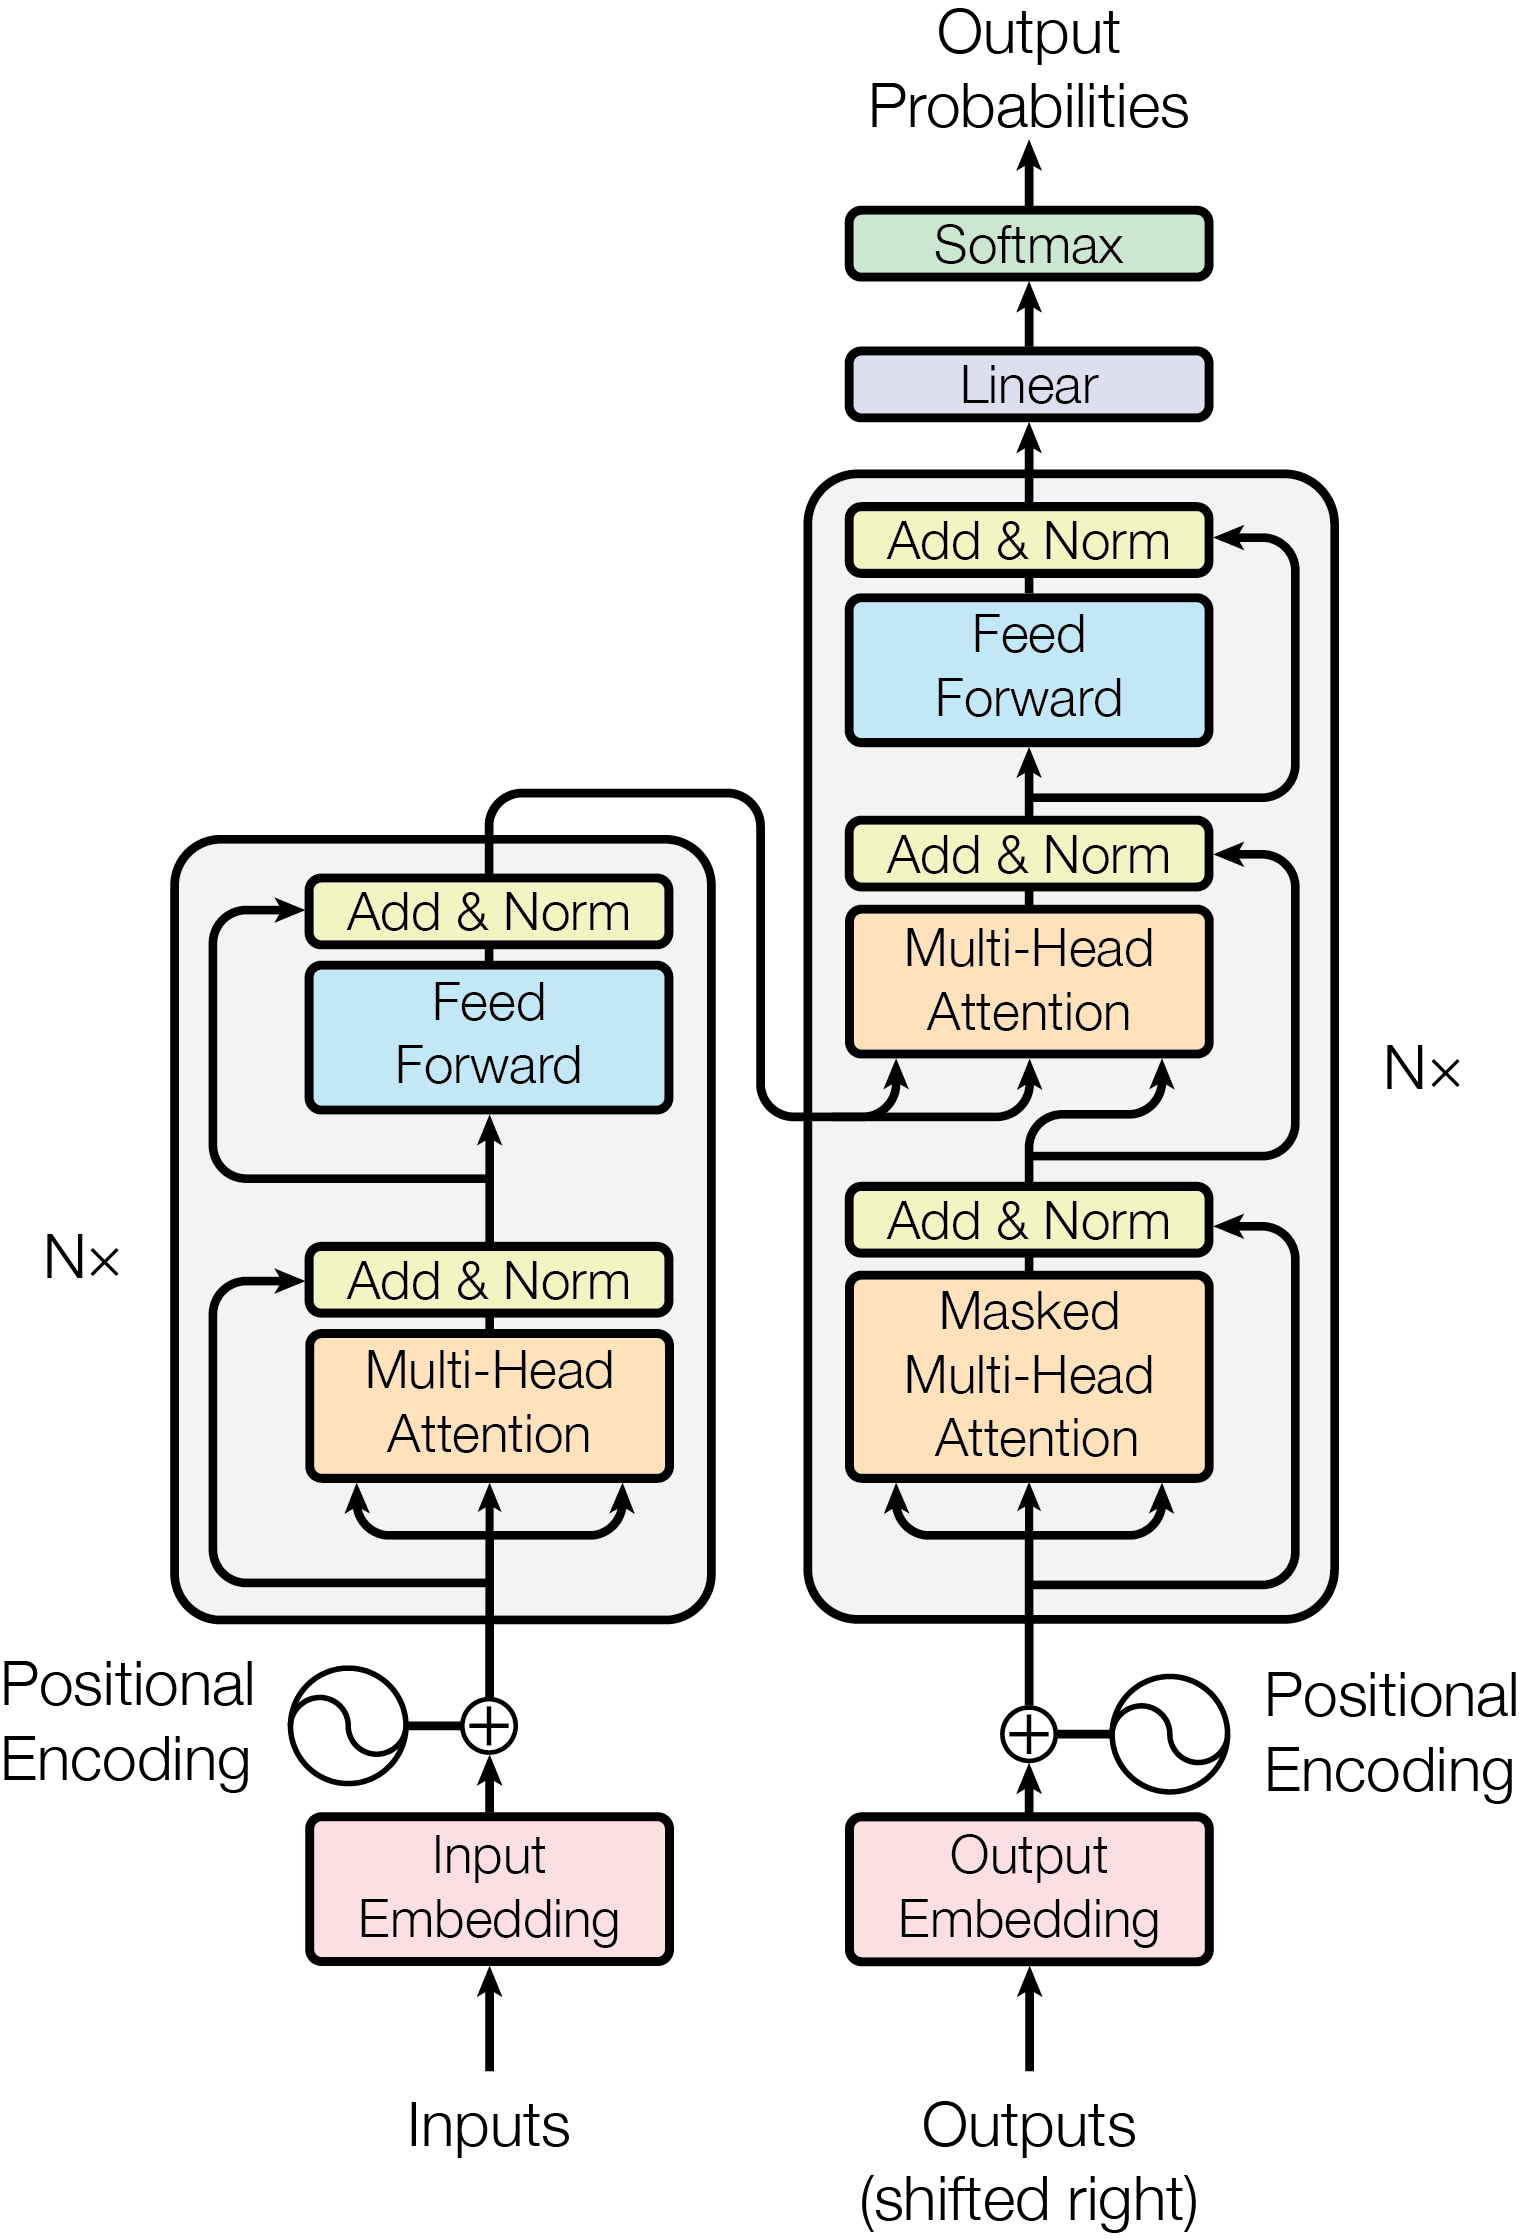
\includegraphics[width=0.5\linewidth]{gambar/ModalNet-21.png}
    \caption{Arsitektur Transformer}
    \label{fig:transformer}
\end{figure}

\subsection{\textit{Positional Encoding}}
Arsitektur Transformer bersifat paralel sehingga diperlukan \textit{Positional Encoding} untuk memberikan informasi urutan pada \textit{sequence}. \textit{Positional Encoding} memiliki ukuran dimensi yang sama dengan \textit{embedding} input sehingga dapat dijumlahkan. Positional encoding dijelaskan pada \ref{subsubsec:pos_enc_sin} dan \ref{subsubsec:trainable_embedding}.

\subsubsection{\textit{Positional encoding sinusoidal}}
\label{subsubsec:pos_enc_sin}
\begin{equation}
    PE_{(pos, 2i)} = \sin \left(pos / 10000^{2i/d_{\text{model}}}\right)
    \label{eq:1}
\end{equation}
\begin{equation}
    PE_{(pos, 2i+1)} = \cos \left(pos / 10000^{2i/d_{\text{model}}}\right)
    \label{eq:2}
\end{equation}

Keterangan:
\begin{itemize}
    \item $PE_{(pos, 2i)}$ adalah posisi pada indeks ganjil
    \item $PE_{(pos, 2i+1)}$ adalah posisi pada indeks genap
    \item $pos$ adalah posisi sampel/data dalan \textit{sequence}
    \item $i$ adalah dimensi data
    \item $d_{\text{model}}$ adalah ukuran embedding
\end{itemize}
$pos$ merupakan posisi dan $i$ merupakan dimensi. $2i$ dan $2i+1$ adalah indeks ganjil dan genap dalam embedding. \textit{Positional encoding sinusoidal} dipilih karena memungkinkan model untuk mengekstrapolasi \textit{sequnece} yang lebih panjang daripada yang ditemui selama pelatihan.

\subsubsection{Trainable Embedding}
\label{subsubsec:trainable_embedding}
\textit{Trainable Embedding} banyak digunakan pada \textit{Large Language Model} (LLM) seperti BERT \cite{devlin2019bertpretrainingdeepbidirectional} dan GPT \cite{radford2019language}. \textit{Trainable Embedding} dapat memahami konteks data lebih baik karena nilainya di-update selama proses pelatihan. Pemahaman kontekstual ini membuat \textit{Trainable embedding} jauh lebih optimal dalam tugas-tugas Deep Learning yang kompleks karena dapat memahami pola yang mungkin terlewatkan oleh \textit{Embedding Statis}.

\subsection{\textit{Attention Mechanism}}
Fungsi \textit{Attention} dapat dideskripsikan sebagai pemetaan \textit{Query} dan sekumpulan pasangan \textit{Key-Value} ke suatu \textit{Output}, di mana \textit{Query}, \textit{Key}, \textit{Value}, dan \textit{Output} semuanya merupakan vektor. \textit{Self-Attention} menghubungkan semua posisi dengan jumlah operasi \textit{sequence} yang konstan sehingga mempercepat operasi dibandingkan layer recurrent pada RNN. Fungsi \textit{Attention} dijelaskan pada persamaan \ref{eq:attention}
% Requires: \usepackage{amsmath}
\begin{equation}
    \text{Attention}(Q, K, V) = \text{softmax}\left(\frac{QK^T}{\sqrt{Head\_DIM}}\right)V
    \label{eq:attention}
\end{equation}
Keterangan:
\begin{itemize}
    \item $\text{Attention}(Q, K, V)$ adalah mekanisme \textit{self-attention}
    \item $Q$ adalah \textit{Query}
    \item $K$ adalah \textit{Key}
    \item $V$ adalah \textit{Value}
    \item $Head\_DIM$ adalah dimensi embedding
\end{itemize}

\textit{Multi-Head Attention} memungkinkan model untuk secara bersamaan memberikan \textit{Attention} informasi dari subruang representasi yang berbeda pada posisi yang berbeda \ref{eq:multi_head_attention}.

\begin{equation}
\begin{aligned}
    \text{MultiHead}(Q, K, V) &= \text{concat}(\text{head}_1, \ldots, \text{head}_h) W^O \\
    \text{dengan head}_i &= \text{Attention}(Q W^Q_i, K W^K_i, V W^V_i)
\end{aligned}
\label{eq:multi_head_attention}
\end{equation}
Keterangan:
\begin{itemize}
    \item $\text{MultiHead}(Q, K, V)$ adalah mekanisme multi-head attention
    \item $\text{head}_i$ adalah mekanisme attention
    \item $W^Q_i$ adalah bobot untuk \textit{Query}
    \item $W^K_i$ adalah bobot untuk \textit{Key}
    \item $W^V_i$ adalah bobot untuk \textit{Value}
    \item $W^O$ adalah bobot untuk multi-head attention
\end{itemize}

\subsection{\textit{Position-wise Feed-Forward Networks}}
Masing-masing lapisan dalam encoder dan decoder terdapat \textit{Feed-Forward Networks} yang saling terhubung, yang diterapkan ke setiap posisi secara terpisah dan identik. Fungsi \textit{Feed-Forward Networks} dapat dilihat pada persamaan \ref{eq:ffn}.

\begin{equation}
   \text{FFN}(x) = \max(0, xW_1 + b_1)W_2 + b_2
   \label{eq:ffn}
\end{equation}
Keterangan:
\begin{itemize}
    \item $\text{FFN}(x)$ adalah mekanisme Feed-Forward Networks
    \item $x$ adalah nilai input neuron
    \item $W_1$ adalah bobot pertama
    \item $b_1$ adalah bias pertama
    \item $W_2$ adalah bobot kedua
    \item $b_2$ adalah bobot kedua
\end{itemize}

Meskipun transformasi linier sama di berbagai posisi, FNN menggunakan parameter yang berbeda pada setiap lapisan.
\subsection{\textit{Layer Nornalization}}
\textit{Layer Normalization} digunakan untuk menormalkan output dari setiap jaringan, sehingga distribusi nilainya stabil selama \textit{training} \ref{eq:layer_normalization}. Parameter $\gamma$ dan $\beta$ merupakan parameter pelatihan dan $\epsilon$ merupakan nilai konstan $10^{-6}$.
\begin{equation}
    \text{LayerNorm}(x) = \frac{x - \mu}{\sqrt{\sigma^2 + \epsilon}} \cdot \gamma + \beta
    \label{eq:layer_normalization}
\end{equation}
Keterangan:
\begin{itemize}
    \item $\text{LayerNorm}(x)$ adalah Layer Normalisasi
    \item $x$ adalah nilai input layer
    \item $\mu$ adalah rataan
    \item $\sigma^2$ adalah standar deviasi
    \item $\epsilon$ adalah nilai galat agar pembagi tidak bernilai $0$
    \item $\gamma \text{ dan } \beta$ adalah parameter pelatihan
\end{itemize}
% Vision Transformer
\section{\textit{Video Vision Transformer}}
Pada ViViT, video input $V$ dengan dimensi $D$ (depth), $H$ (tinggi), $W$ (lebar), dan $C$ (channel) dibagi-bagi menjadi potongan-potongan kecil yang disebut \textit{patch}\cite{arnab2021vivitvideovisiontransformer}. Setiap \textit{patch} $P$ memiliki dimensi $P_d \times P_h \times P_w \times C$.
Proses pembagian video menjadi \textit{patch} ini dapat divisualisasikan sebagai persamaan \ref{eq:reshape}
\begin{equation}
   V \in \mathbb{R}^{D \times H \times W \times C} \rightarrow \text{Reshape} \rightarrow P \in \mathbb{R}^{N \times (P_d \times P_h \times P_w \times C)}
   \label{eq:reshape}
\end{equation}
Keterangan:
\begin{itemize}
    \item $V$ adalah input embedding video
    \item $P$ adalah input patch embedding
    \item $\text{Reshape}$ adalah mengubah input video ke patch
    \item $D$ adalah ukuran \textit{depth} kedalaman/frame
    \item $H$ adalah ukuran \textit{height} atau tinggi
    \item $W$ adalah ukuran \textit{width} atau lebar
    \item $C$ adalah jumlah $channel$ atau kanal
\end{itemize}

di mana $N = (D/P_d) \times (H/P_h) \times (W/P_w)$ adalah jumlah total \textit{patch} yang dihasilkan.
Selanjutnya, setiap \textit{patch} $P$ diproyeksikan ke dalam ruang \textit{embedding} dengan dimensi $d$ melalui sebuah lapisan linear. Hasil proyeksi ini membentuk sebuah \textit{sequence} token $Z$ dengan dimensi $N \times d$ sesuai persamaan \ref{eq:linear_map}
\begin{equation}
    Z = \text{Linear}(P) \in \mathbb{R}^{N \times d} \label{eq:linear_map}
\end{equation}
Keterangan:
\begin{itemize}
    \item $Z$ adalah hasil proyeksi \textit{patch embedding}
    \item $P$ adalah \textit{patch embedding}
\end{itemize}

\textit{Sequence} token $Z$ ditambahkan dengan \textit{positional encoding} yang  kemudian menjadi input untuk \textit{encoder transformer}. Terdapat dua metode utama untuk menghasilkan \textit{patch embedding} yaitu, \textit{Uniform Frame Sampling} yang hanya memiliki informasi spasial dan \textit{Tubelet Embedding} yang menghasilkan \textit{patch} yang mencakup informasi spasial dan temporal.

% Bab 3 metodologi penelitian
\chapter{METODE PENELITIAN}

\section{Deskripsi Data}
Dataset yang digunakan adalah \textit{Medical Sound Classification Challenge} yang diselenggarakan oleh Himanshu Kaushik pada platform Kaggle\cite{airs-ai-in-respiratory-sounds}. Dataset ini memiliki 882 jumlah data yang terdiri dari tiga jenis data untuk setiap individu yaitu audio batuk, vowel dan fitur riwayat pasien. Data diidentifikasi menggunakan candidateID yang ditetapkan untuk setiap orang. File suara dan embedding terdapat di folder candidateID yang diberikan. Dataset terbagi menjadi dua jenis yaitu 544 untuk data latih dan 338 untuk data uji yang belum memiliki label. Label penyakit terdiri dari 3 kelas yaitu asma, COPD dan pasien sehat.
\begin{figure}[H]
    \centering
    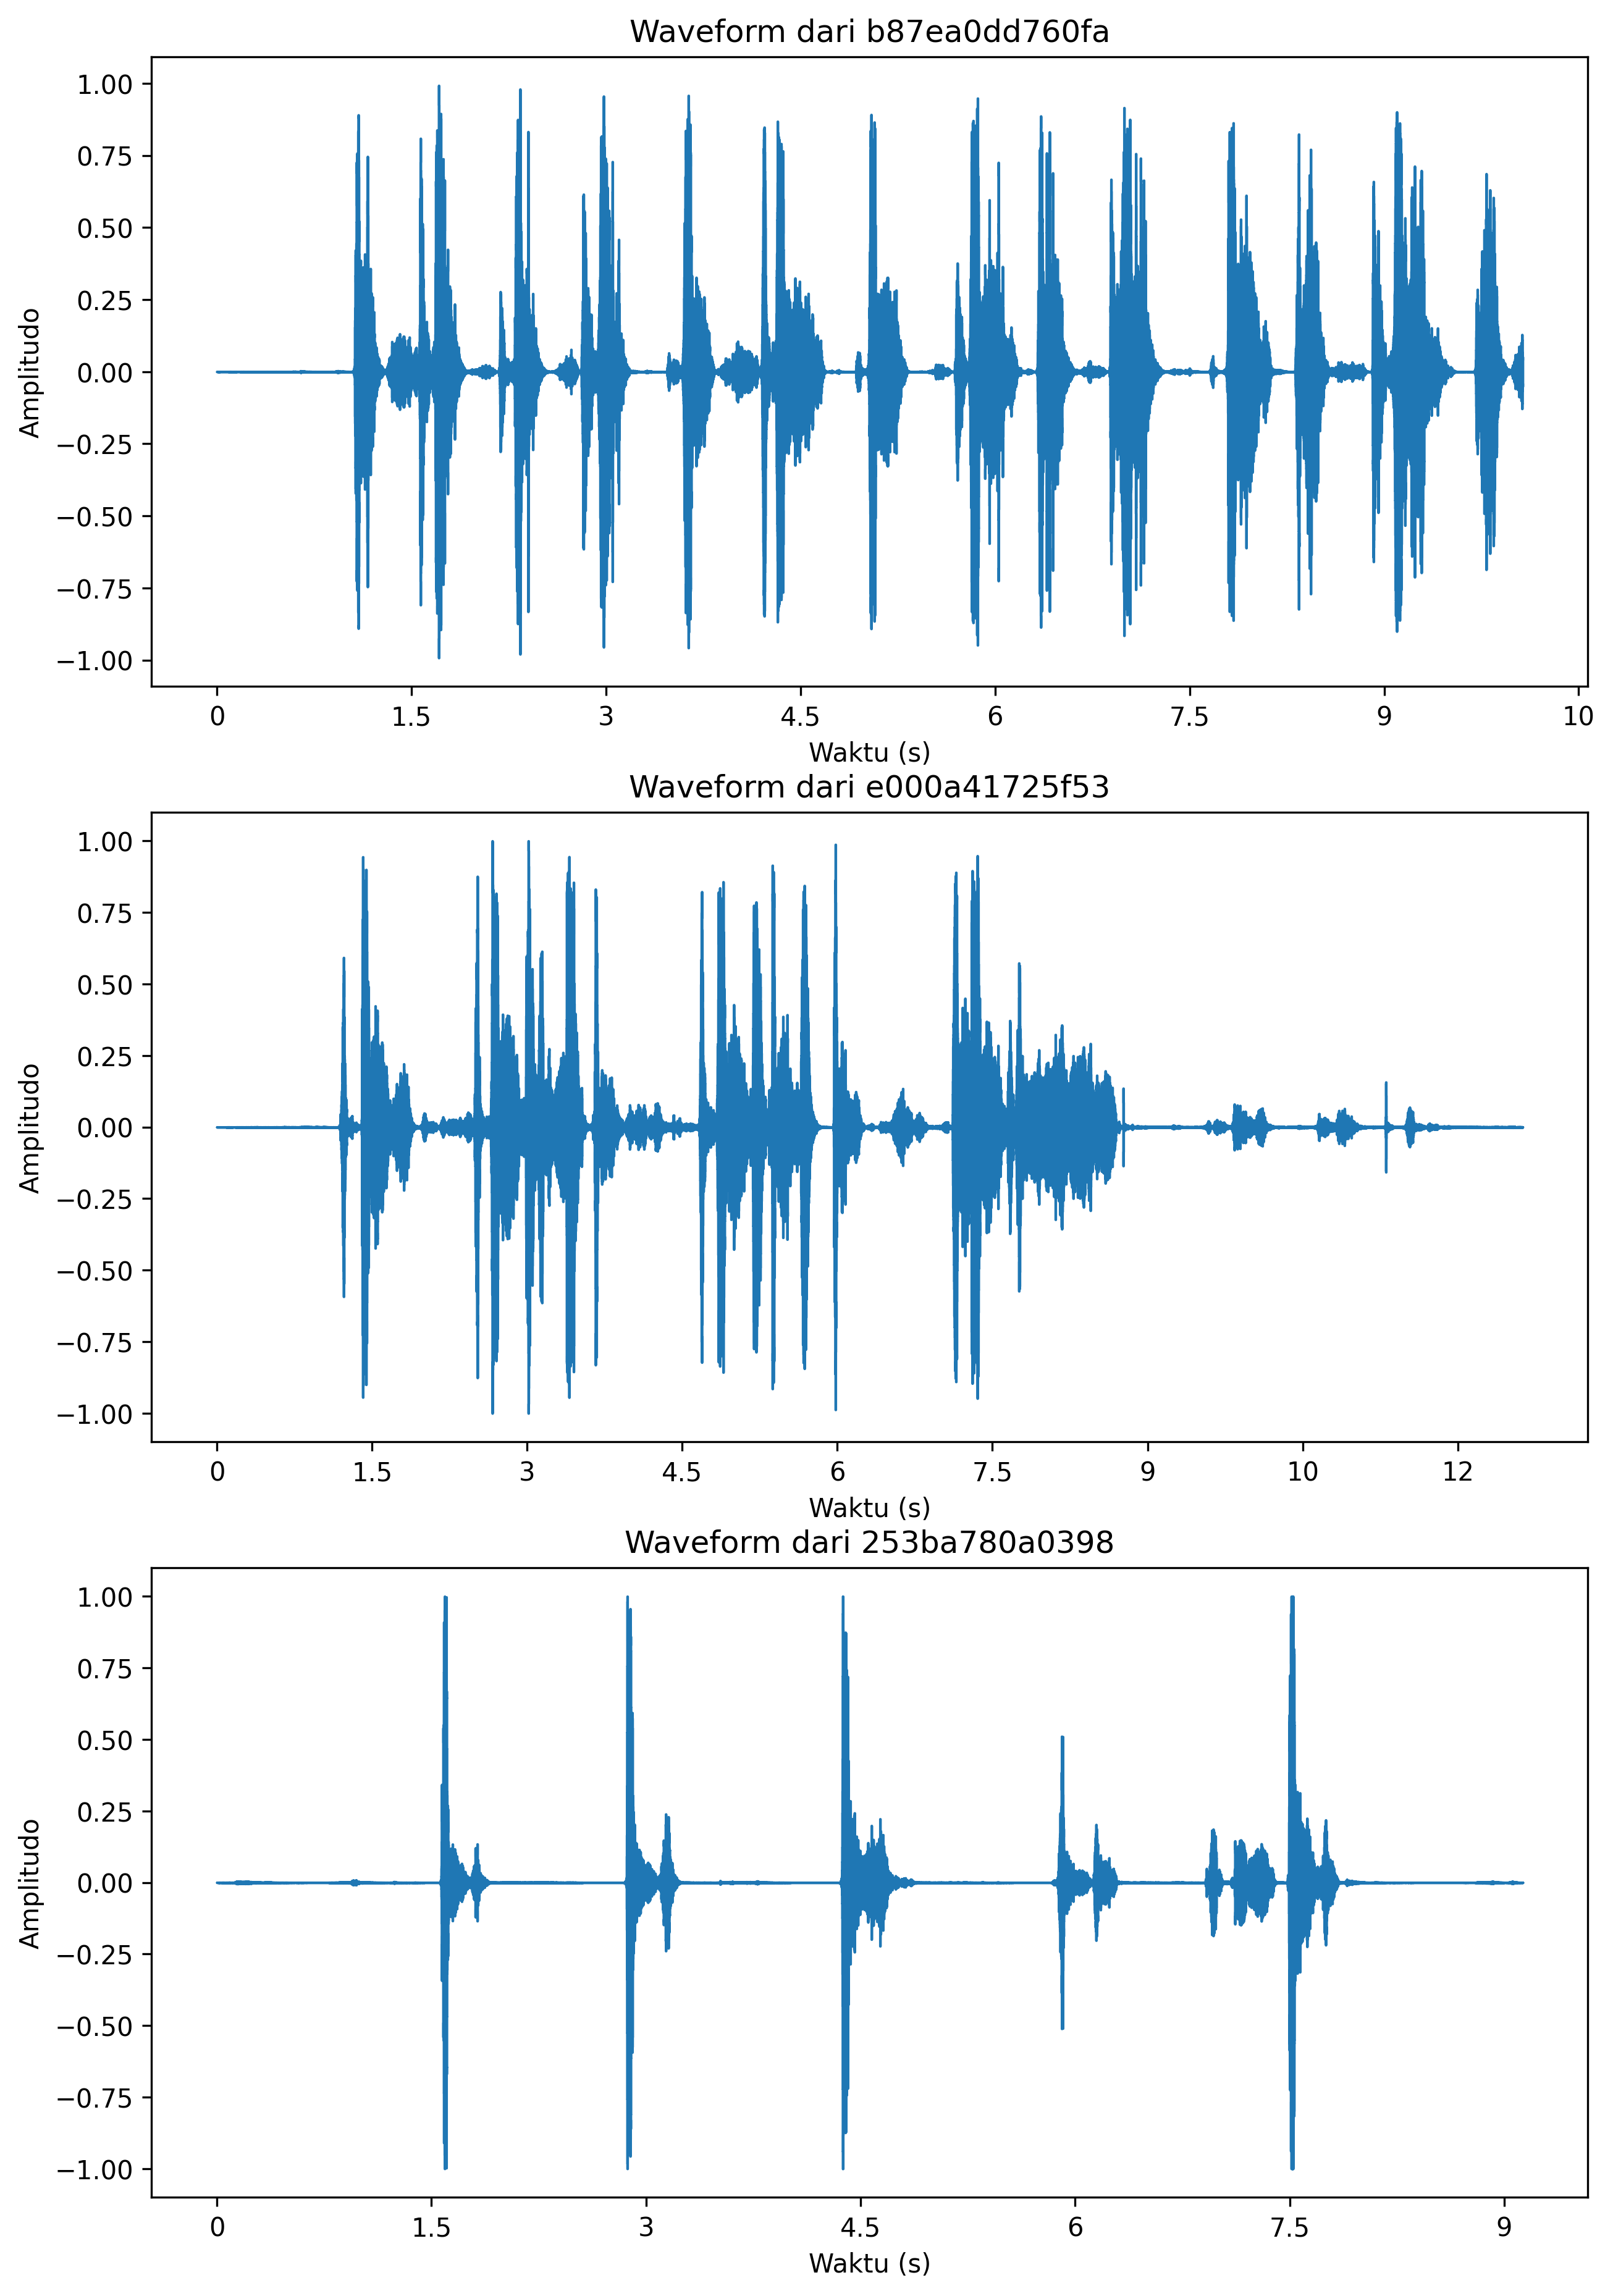
\includegraphics[width=0.7\linewidth]{gambar/waveforms.png}
    \caption{Visualisasi gelombang suara tiap kelas}
    \label{fig:waveform}
\end{figure}

\begin{landscape}
\begin{longtable}{p{3cm}lcccccccccc}
\caption{Tabel riwayat pasien}\\
\hline
\textbf{candidateID} & \textbf{age} & \textbf{gender} & \textbf{tbContact} & \textbf{wheezing} & \textbf{phlegmCough} & \textbf{familyAsthma} & \textbf{feverHistory} & \textbf{coldPresent} & \textbf{packYears} & \textbf{disease} \\ \hline
%\endfirsthead

%\multicolumn{4}{l}{\bfseries \tablename\ \thetable{} -- Lanjutan dari halaman sebelumnya}\\
% \begin{center}
% % {{\bfseries \tablename\ \thetable{} -- Lanjutan dari halaman sebelumnya}} \\
% \end{center}
%\hline
%\textbf{candidateID} & \textbf{age} & \textbf{gender} & \textbf{tbContact} & \textbf{wheezing} & \textbf{phlegmCough} & \textbf{familyAsthma} & \textbf{feverHistory} & \textbf{coldPresent} & \textbf{packYears} & \textbf{disease} \\ \hline

%\endhead

%\hline
%\endfoot

%\endlastfoot

2bbd6c5ecf1ce & 55 & 1 & 0.0 & 0.0 & 0.0 & 1.0 & 0.0 & 0.0 & 0 & 1 \\
75fa6e335b5ca & 65 & 0 & 0.0 & 1.0 & 0.0 & 0.0 & 0.0 & 1.0 & 560 & 2 \\
7dc99cfcb5aa & 43 & 0 & 0.0 & 1.0 & 0.0 & 0.0 & 0.0 & 0.0 & 0 & 1 \\
59cf4a7821471 & 74 & 0 & 0.0 & 1.0 & 0.0 & 0.0 & 0.0 & 0.0 & 800 & 2 \\
59f9fe56c2f12 & 28 & 0 & 0.0 & 0.0 & 1.0 & 0.0 & 0.0 & 0.0 & 0 & 0 \\
caee891a86d8d & 56 & 1 & 0.0 & 1.0 & 0.0 & 0.0 & 0.0 & 0.0 & 0 & 1 \\
5b8578b39385f & 31 & 0 & 0.0 & 0.0 & 1.0 & 0.0 & 0.0 & 0.0 & 0 & 0 \\
f3e7d50ce7288 & 35 & 0 & 0.0 & 1.0 & 1.0 & 0.0 & 0.0 & 0.0 & 0 & 1 \\
ad5fa122d4efb & 56 & 1 & 0.0 & 0.0 & 0.0 & 1.0 & 0.0 & 0.0 & 0 & 0 \\
14b58d18c66c7 & 57 & 0 & 0.0 & 1.0 & 1.0 & 0.0 & 0.0 & 0.0 & 0 & 0 \\
7959121db060d & 48 & 0 & 0.0 & 1.0 & 0.0 & 0.0 & 0.0 & 0.0 & 0 & 1 \\
77aa6a34f6da1 & 21 & 0 & 0.0 & 0.0 & 1.0 & 1.0 & 0.0 & 0.0 & 0 & 1 \\
069276518f6f & 25 & 1 & 0.0 & 0.0 & 0.0 & 1.0 & 0.0 & 0.0 & 0 & 2 \\
3d71862ec1801 & 48 & 1 & 0.0 & 0.0 & 1.0 & 1.0 & 0.0 & 0.0 & 0 & 1 \\
1868d92d2db4 & 20 & 0 & 0.0 & 0.0 & 0.0 & 1.0 & 0.0 & 1.0 & 360 & 2 \\
fbf8398bd0136 & 70 & 0 & 0.0 & 0.0 & 1.0 & 0.0 & 0.0 & 0.0 & 0 & 1 \\
0343c366074ec & 25 & 0 & 0.0 & 1.0 & 1.0 & 0.0 & 0.0 & 0.0 & 0 & 1 \\ 
\dots & \dots & \dots & \dots & \dots & \dots & \dots & \dots & \dots & \dots & \dots \\ 
e17cb00bd9677 & 66 & 0 & 0.0 & 0.0 & 1.0 & 0.0 & 0.0 & 1.0 & 0 & 2 \\
\hline
\label{table:riwayat_pasien}
\end{longtable}
\end{landscape}

\section{Rancangan Penelitian}
\begin{figure}[H]
    \centering
    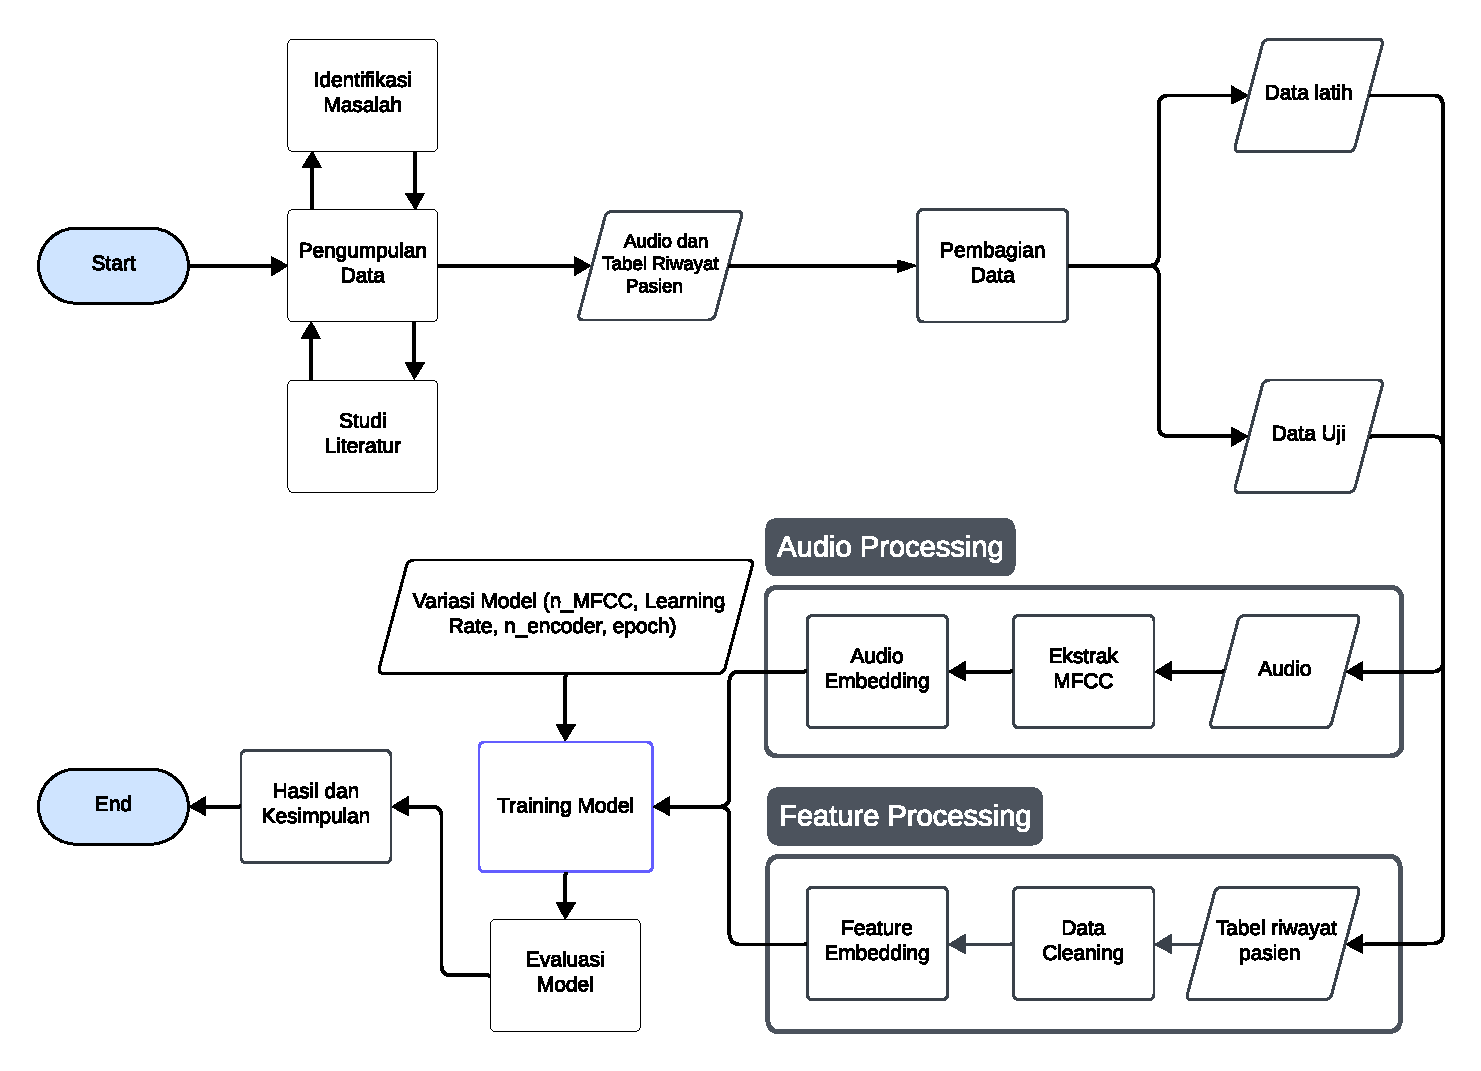
\includegraphics[width=1\linewidth]{gambar/Flowchart Rancangan Penelitian.pdf}
    \caption{\textit{Flowchart} rancangan penelitian}
    \label{fig:flowchart}
\end{figure}

    \subsection{Pengumpulan Data}
    Data diunduh ke dalam \textit{notebook} menggunakan kaggle-api dengan fungsi yang telah disediakan di laman kompetisi. File unduhan berupa .zip yang harus diekstrak terlebih dahulu.

    \subsection{Pembagian Data}
    Data dibagi menjadi data latih dan data uji dengan perbandingan 80\% untuk data latih dan 20\% untuk data uji. Digunakan parameter random state agar proses pembagian data bisa direproduksi ulang. Dilakukan \textit{stratified sampling} berdasarkan kolom target yaitu \textit{disease} untuk memastikan distribusi kelas tetap sama di kedua set.

    \subsection{Pemrosesan Suara}
    Data suara yang digunakan pada penelitian ini berupa suara batuk \textit{cough.wav} pasien yang berisi minimal 3 kali batuk, dengan durasi rekaman maksimal 15 detik. Dilakukan ekstraksi fitur menggunakan \textit{Mel frequency Capstral Coefficients} (MFCC), yaitu dengan cara memfilter secara logaritmik pada frekuensi di atas 1000 Hz dan secara linier pada frekuensi di bawah 1000 Hz. MFCC dapat meningkatkan sensitivitas pada suara dengan frekuensi rendah dan sebaliknya, pada suara dengan frekuensi tinggi MFCC dapat mengurangi sensitivitas dalam menangkap suara \cite{10593181}.
    \begin{algorithm}[H]
    \caption{Ekstraksi MFCC}
    \begin{algorithmic}[1]
    
    \Function{ExtractMFCC}{$file\_path, n\_mfcc, target\_length$}
        \State Load audio file and sampling rate: $(audio, sr) \gets \Call{Load}{file\_path}$
        \State Compute MFCC: $mfcc \gets \Call{ComputeMFCC}{audio, sr, n\_mfcc}$
        \State Transpose $mfcc$: $mfcc \gets mfcc^T$
        \If{$\text{length}(mfcc) > target\_length$}
            \State Trim $mfcc$ to $target\_length$
        \ElsIf{$\text{length}(mfcc) < target\_length$}
            \State Pad $mfcc$ with zeros
        \EndIf
        \State \Return $mfcc$
    \EndFunction
    
    \end{algorithmic}
    \label{algo:audio_process}
    \end{algorithm}

    \subsection{Pemrosesan Data Tabel Riwayat Pasien}
    Dilakukan \textit{preprocessing} seperti pengecekan nilai kosong, penghapusan fitur yang tidak relevan untuk memastikan kualitas data yang baik agar model dapat menangkap informasi yang relevan pada data.
    \begin{algorithm}[H]
    \caption{Pemrosesan Data}
    \begin{algorithmic}[1]
    \Function{PreprocessFeatures}{$row$}
        \State Normalize numerical features
        \State Extract categorical features
        \State Combine all features into a vector
        \State \Return Feature vector
    \EndFunction
    
    \Function{ProcessRow}{$row$}
        \State Get candidate ID: $id \gets row["candidateID"]$
        \State Generate audio path: $audio\_path \gets \Call{Join}{SOUND\_FOLDER, id, "cough.wav"}$
        \State Extract MFCC: $mfcc \gets \Call{ExtractMFCC}{audio\_path}$
        \State Process features: $features \gets \Call{PreprocessFeatures}{row}$
        \State One-hot encode label: $label \gets \Call{OneHotEncode}{row["disease"], depth=3}$
        \State \Return $(mfcc, features, label)$
    \EndFunction
    \end{algorithmic}
    \label{algo:feature_process}
    \end{algorithm}

    \subsection{Pemodelan}
    Pada tahapan ini dilakukan rancangan model yang akan digunakan, seperti desain arsitektur, \textit{loss function}, dan \textit{optimizer} beserta \textit{hyperparameter}-nya. Pada penelitian ini juga akan menggunakan beberapa desain arsitektur yang berfokus pada kedalaman seperti jumlah \textit{block} dan \textit{hyperparameter} jumlah \textit{attention head}.

    \subsection{Arsitektur}
    Penelitian ini akan menggunakan MFCC untuk mengekstraksi fitur audio dan serta \textit{embedding} data riwayat pasien.
    \begin{figure}[H]
        \centering
        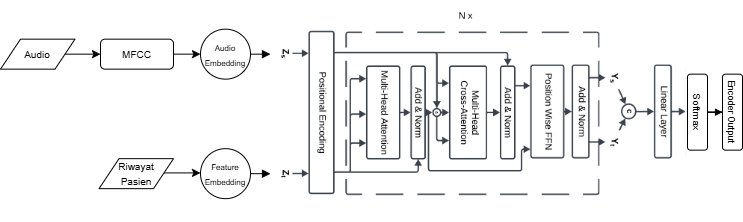
\includegraphics[width=1\linewidth]{gambar/Arsitektur Model.png}
        \caption{Desain rancangan arsitektur model.}
        \label{fig:model}
    \end{figure}
    Input berupa audio dengan fitur MFCC berukuran \(T \times F\) (dengan \(T\) adalah jumlah frame dan \(F\) adalah jumlah koefisien MFCC) dan data riwayat pasien berukuran \(N \times d_{feat}\) (\(N\) adalah jumlah data riwayat, \(d_{feat}\) adalah dimensi fitur) akan diubah menjadi embedding berukuran \(T \times d_{embed}\) dan \(N \times d_{embed}\) melalui \textit{embedding layer}. \textit{Embedding} ini ditambahkan dengan \textit{positional encoding} dan diteruskan ke \textit{encoder} berbasis transformer, di mana mekanisme \textit{self-attention} dan \textit{cross-attention} digunakan untuk menangkap hubungan antar fitur audio serta interaksi antara audio dan riwayat pasien. Setelah melalui \textit{feedforward network} (FFN), hasil akhir \textit{encoder} berupa \textit{embedding multimodal} dikombinasikan dan diproyeksikan menggunakan linear layer, diikuti oleh \textit{softmax} untuk menghasilkan output akhir dari token [cls] berupa representasi yang dapat digunakan untuk klasifikasi.

    \subsection{\textit{Loss Function}}
    Fungsi kerugian yang digunakan \textit{Categorical Cross-Entropy} untuk setiap kelas \ref{eq:cross_entropy}:
    \begin{equation}
        L(y, \hat{y}) = -\sum_{i=1}^{C} y_i \log(\hat{y}_i)
    \label{eq:cross_entropy}
    \end{equation}
    Keterangan:
    \begin{itemize}
        \item $L(y, \hat{y})$ adalah nilai \textit{Categorical Cross-Entropy}
        \item $y$ adalah nilai target asli
        \item $\hat{y}_i$ adalah nilai prediksi
    \end{itemize}
    
    Di mana $L(y, \hat{y})$ merupakan \textit{categorical cross-entropy loss}. $y_i$ adalah label sebenarnya (0 atau 1 untuk setiap kelas) dari \textit{one-hot encoding} vektor target. $\hat{y}_i$ adalah probabilitas yang diprediksi untuk kelas $i$. $C$ merupakan jumlah kelas yang diprediksi.

    \subsection{Pelatihan Model}
    Penelitian ini akan menggunakan \textit{optimizer} sama dengan yang digunakan Vaswani et al., yaitu \textit{optimizer} Adam \cite{ahn2024understandingadamoptimizeronline} yang menggabungkan momentum dengan RMSprop. Model akan dilatih menggunakan \textit{Notebook Kaggle} dengan GPU NVIDIA Tesla P100-PCIE-16GB untuk model \textit{small} dan \textit{big}. Beberapa kedalaman \textit{layer} dan jumlah \textit{head attention} akan diuji performanya dengan tetap memperhatikan batasan komputasi.
\begin{algorithm}[H]
    \caption{Pelatihan Model}
    \begin{algorithmic}[1]
        \State \textbf{Inisialisasi:} $m_0 \gets 0, v_0 \gets 0, t \gets 0, \beta_1 \gets 0.9, \beta_2 \gets 0.98, \epsilon \gets 10^{-9}$
        \State \textbf{Inisialisasi:} epochs, batch\_size
        \While{epoch $\to$ epochs}
            \While{step $\to$ N // batch\_size}
                \State $lr \gets (d_{embed}^{-0.5} \cdot min(step^{-0.5}, \, step \times    4000^{-1.5}))$
                \State $t \gets t + 1$
                
                \State $g_t \gets \nabla_\theta \mathcal{L}(\theta_{t-1}) \quad \text{(Gradien  \textit{loss function})}$
                
                \State $m_t \gets \beta_1 \cdot m_{t-1} + (1 - \beta_1) \cdot g_t \quad     \text{(Update momentum pertama)}$
                
                \State $v_t \gets \beta_2 \cdot v_{t-1} + (1 - \beta_2) \cdot g_t^2 \quad   \text{(Update momentum kedua)}$
                
                \State $\hat{m}_t \gets m_t / (1 - \beta_1^t) \quad \text{(Koreksi bias     momentum pertama)}$
    
                \State $\hat{v}_t \gets v_t / (1 - \beta_2^t) \quad \text{(Koreksi bias     momentum kedua)}$
    
                \State $\theta_{t} \gets \theta_{t-1} - lr \cdot \hat{m}_t / (\sqrt{\hat{v}_t +     \epsilon}) \quad \text{(Update parameter)}$
            \EndWhile
        \EndWhile
        \State \textbf{\textit{Return}:} Parameter $\theta_t$
    \end{algorithmic}
\end{algorithm}


\section{Evaluasi Model}
	\subsection{\textit{Confusion Matrix}}
    \textit{Confussion matrix} adalah metode dalam pembelajaran mesin yang menyediakan representasi visual dari performa model dalam tugas klasifikasi \cite{10708595}. Matriks ini merangkum prediksi yang benar dan salah yang dibuat oleh model, yang memungkinkan penghitungan berbagai metrik kinerja seperti akurasi, presisi, \textit{recall}, dan \textit{F1-score}. Matriks ini biasanya terdiri dari empat komponen: \textit{True Positive}, \textit{True Negarive}, \textit{False Positive}, dan \textit{False Negative} \ref{tab:confusion_matrix_and_metrics}.
    
    \begin{table}[h]
        \centering
        \caption{\textit{Confusion Matrix} untuk 3 Kelas (a), Rumus metrik evaluasi (b)}
        \begin{minipage}{0.5\textwidth}
          \centering
          \begin{tabular}{c c c c c}
            \hline
            \multicolumn{2}{c}{\textbf{Actual Class}} & \multicolumn{3}{c}{\textbf{Predicted Class}} \\
            \hline
            \multicolumn{2}{c}{} & \cellcolor{gray!20}$C_1$ & \cellcolor{gray!20}$C_2$ &    \cellcolor{gray!20}$C_3$ \\
            \multirow{3}{*}{\rotatebox{90}{\textbf{Actual}}} 
            & \cellcolor{gray!20}$C_1$ & \cellcolor{green!20}TP$_{1}$ & FP$_{12}$ & FP$_{13}$ \\
            
            & \cellcolor{gray!20}$C_2$ & FN$_{21}$ & \cellcolor{green!20}TP$_{2}$ & FP$_{23}$ \\
            
            & \cellcolor{gray!20}$C_3$ & FN$_{31}$ & FN$_{32}$ & \cellcolor{green!20}TP$_{3}$ \\
            \hline
          \end{tabular}
          \subcaption{}
        \end{minipage}%
        \begin{minipage}{0.5\textwidth}
          \centering
          \begin{tabular}{l l}
          \hline
          \textbf{Metrik} & \textbf{Rumus} \\
          \hline\\
          Accuracy & $\frac{TP + TN}{TP + TN + FP + FN}$ \\
          \\
          Precision & $\frac{TP}{TP + FP}$ \\
          \\
          Recall & $\frac{TP}{TP + FN}$ \\
          \\
          F1-Score & $2 \times \frac{\text{Precision} \times \text{Recall}}{\text{Precision} +  \text{Recall}}$ \\\\
          \hline
          \end{tabular}
          \subcaption{}
        \end{minipage}
        \label{tab:confusion_matrix_and_metrics}
    \end{table}
    
    \subsection{Kurva ROC-AUC}
    Kurva ROC-AUC merupakan metode untuk mengevaluasi keakuratan algoritma klasifikasi, yang memberikan wawasan tentang kinerjanya di berbagai ambang batas. Kurva ini mengukur keseimbangan antara sensitivitas (\textit{true positive rate}) dan spesifisitas (\textit{false positive rate}), yang memungkinkan penilaian komprehensif terhadap efektivitas model \cite{10420319}.
    % Requires: \usepackage{amsmath}
\begin{equation}
   \text{TPR/sensitivitas} = \frac{\text{TP}}{\text{TP} + \text{FN}}
   \label{eq:tpr}
\end{equation}
\begin{equation}
   \text{FPR/spesifisitas} = \frac{\text{FP}}{\text{FP} + \text{TN}}
   \label{eq:fpr}
\end{equation}
\begin{figure}[H]
    \centering
    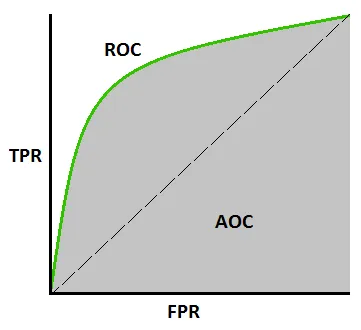
\includegraphics[width=0.4\linewidth]{gambar/ROC-AUC.png}
    \caption{Kurva ROC-AUC}
    \label{fig:roc_auc}
\end{figure}
% Baris ini digunakan untuk membantu dalam melakukan sitasi
% Karena diapit dengan comment, maka baris ini akan diabaikan
% oleh compiler LaTeX.
\begin{comment}
\bibliography{daftar-pustaka}
\end{comment}


% Bab 4 hasil dan pembahasan
\chapter{HASIL DAN PEMBAHASAN}

\section{Persiapan \textit{Workspace Kaggle Notebook}}
\subsection{Buat \textit{Notebook Kaggle}}
\begin{figure}[H]
    \centering
    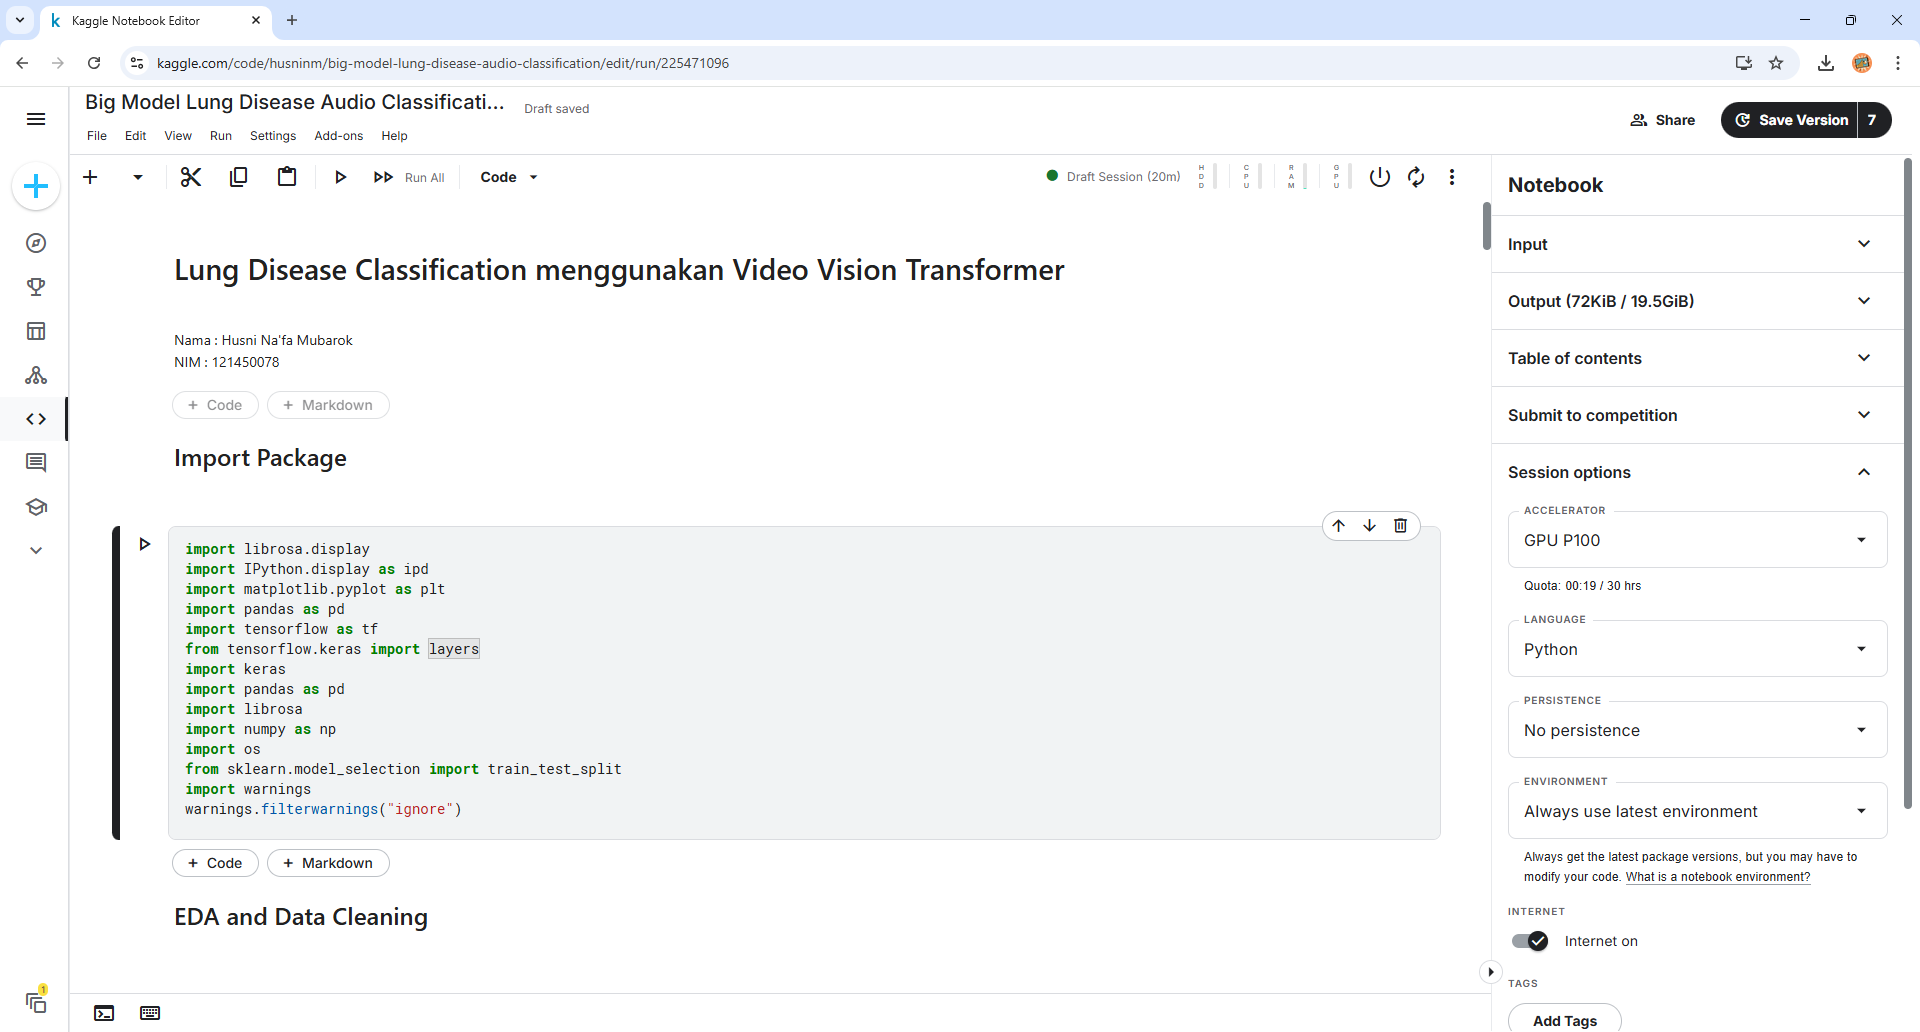
\includegraphics[width=1\linewidth]{gambar/Screenshot 2025-03-10 103758.png}
    \caption{\textit{Kaggle Workspace}}
    \label{fig:kaggle_workspace}
\end{figure}
\subsection{Import Package/Library yang digunakan}
\begin{table}[H]
    \centering
    \caption{Daftar Library Python dan Deskripsinya}
    \begin{tabular}{l p{8cm}}
        \hline
        \textbf{Library} & \textbf{Deskripsi} \\ \hline
        \texttt{librosa} & Digunakan untuk analisis dan pemrosesan audio, seperti ekstraksi fitur suara. \\
        \texttt{librosa.display} & Modul dari \texttt{librosa} untuk menampilkan dan memvisualisasikan data audio. \\
        \texttt{IPython.display} & Menyediakan fungsi untuk menampilkan media interaktif, seperti audio dan video di notebook Jupyter. \\
        \texttt{matplotlib.pyplot} & Digunakan untuk membuat visualisasi data, termasuk grafik dan diagram. \\
        \texttt{pandas} & Library untuk manipulasi dan analisis data dalam bentuk tabel (DataFrame). \\
        \texttt{tensorflow} & Framework untuk machine learning dan deep learning. \\
        \texttt{tensorflow.keras.layers} & Modul dari Keras dalam TensorFlow untuk membangun arsitektur jaringan saraf. \\
        \texttt{keras} & High-level API untuk membangun dan melatih model deep learning. \\
        \texttt{numpy} & Digunakan untuk komputasi numerik dan operasi array multidimensi. \\
        \texttt{os} & Modul standar Python untuk berinteraksi dengan sistem file dan direktori. \\
        %\texttt{sklearn.model_selection} & Modul dari \texttt{scikit-learn} yang digunakan untuk membagi dataset menjadi data latih dan uji. \\
        \texttt{warnings} & Modul untuk menangani dan menyembunyikan peringatan di Python. \\ \hline
    \end{tabular}
    \label{tab:library_python}
\end{table}

\section{\textit{Exploratory data analysis} dan \textit{Data Cleaning}}

\section{Pembagian Data \textit{(Data Splitting)}}
Data dibagi dengan perbandingan 80:20

\section{Pembuatan Pipeline \textit{Data Processing}}

\subsection{\textit{Audio Processing}}
Data suara diekstrak menggunakan ekstraksi fitur MFCC.
% \begin{table}[H]
% \centering
% \caption{Parameter kelulusan tugas akhir}
% \begin{tabular}{ clc }
% \hline
% \textbf{No.} & \textbf{Parameter } & \textbf{Nilai} \\
% \hline
% 1. & Penulisan & A \\
% 2. & Penulisan & A \\
% \hline
% \end{tabular}
% \label{table:nilai}
% \end{table}

\subsection{Feature Processing}
Berikut algoritma pemrosesan riwayat pasien \ref{algo:feature_process}


\subsection{Data Generator}
\begin{algorithm}[H]
\caption{PipeLine Model}
\begin{algorithmic}[1]

\Function{DataGenerator}{$data$}
    \ForAll{$row \in data$}
        \State $(mfcc, features, label) \gets \Call{ProcessRow}{row}$
        \State \Yield $(mfcc, features, label)$
    \EndFor
\EndFunction

\Function{CreateDataset}{$data, batch\_size$}
    \State Define dataset signature
    \State Create dataset using \Call{DataGenerator}{$data$}
    \State Batch, shuffle, and prefetch dataset
    \State \Return Dataset
\EndFunction

\Function{SplitData}{$data, test\_size, random\_state$}
    \State Split dataset into train and validation sets
    \State \Return $(train\_data, valid\_data)$
\EndFunction

\State $(train\_data, valid\_data) \gets \Call{SplitData}{data, 0.2, 25}$
\State $train\_dataset \gets \Call{CreateDataset}{train\_data, BATCH\_SIZE}$
\State $valid\_dataset \gets \Call{CreateDataset}{valid\_data, BATCH\_SIZE}$

\end{algorithmic}
\end{algorithm}

% \begin{equation}
%     x+2 = 159
% \end{equation}
% Bla bla bla bla

% %Berikut adalah contoh gambar yang dicetak secara horizontal
% \begin{landscape}
%    \begin{figure}[t]
%         \centering
%         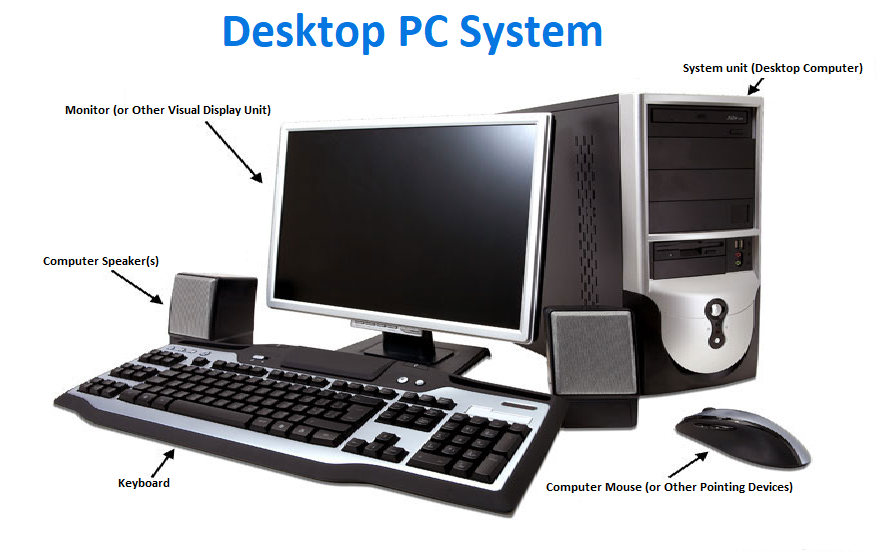
\includegraphics[width=18cm, height=12cm]{gambar/contoh-gambar-miring.png}
%          \caption{Contoh Gambar Komputer}
%         \label{fig:komputer}
%     \end{figure}
% \end{landscape}

\section{Pelatihan Model}
\subsection{Data Pelatihan dan Batching}
\subsection{Optimizer dan Regularisasi}
\subsection{Variasi Model}
\begin{table}[H]
    \centering
    \caption{Variasi parameter untuk model Transformer Small dan Big}
    \begin{tabular}{l|cccccccc|cc}
        \hline
        \textbf{Model} & $N$ & $d_\text{model}$ & $d_\text{ff}$ & $h$ & $d_k$ & $d_v$ & $P_\text{drop}$ & $\epsilon_\text{ls}$ & \textbf{Accuracy} & \textbf{Precision} \\

    \hline\rule{0pt}{2.0ex}
    \multirow{3}{*}{Small}
    & 6 & 32 & & 8 & 512 & 512 & & & 5.29 & 24.9  \\
    & & 64 & & & 128 & 128 & & & 5.00 & 25.5  \\
    & & 128 & & 16 & 32 & 32 & & & 4.91 & 25.8  \\
    \hline\rule{0pt}{2.0ex}
    \multirow{2}{*}{Big}
    & 12 & 64 & & & 16 & & & & 5.16 & 25.1 \\
    & & 128 & & & 32 & & & & 5.01 & 25.4 \\
    \hline
    \end{tabular}
    \label{tab:Variasi_Model}
\end{table}

\subsection{Perbandingan Positional Embedding dengan Trainable Embedding}
\begin{table}[H]
    \centering
    \caption{Perbandingan hasil antara Positional Embedding dan Trainable Embedding.}
    \begin{tabular}{lcc}
        \hline
        \textbf{Metric} & \textbf{Positional Embedding} & \textbf{Trainable Embedding} \\
        \hline
        Accuracy        & 85\%                          & 88\%                         \\
        Precision       & 83\%                          & 86\%                         \\
        Recall          & 82\%                          & 89\%                         \\
        F1-Score        & 82.5\%                        & 87\%                         \\
        \hline
    \end{tabular}
    \label{tab:embedding_comparison}
\end{table}
\section{Evaluasi Model}
\subsection{Akurasi dan Loss Pelatihan}

\subsection{Confussion Matrix}

\subsection{Kurva AUC-ROC}

\subsection{Prediksi Data baru}

% Bab 5 penutup
\chapter{KESIMPULAN DAN SARAN}

\section{Kesimpulan}
Berdasarkan hasil analisis dan pengujian fungsional aplikasi ini, didapat kesimpulan sebagai berikut:

\begin{enumerate}
	\item Lorem ipsum is a pseudo-Latin text used in web design, typography, layout, and printing in place of English to emphasise design elements over content.

	\item It's also called placeholder (or filler) text. It's a convenient tool for mock-ups.

	\item It helps to outline the visual elements of a document or presentation, eg typography, font, or layout. Lorem ipsum is mostly a part of a Latin text by the classical author and philospher Cicero.

	\item Its words and letters have been changed by addition or removal, so to deliberately render its content nonsensical; it's not genuine, correct, or comprehensible Latin anymore.
\end{enumerate}


\section{Saran}
Hal-hal penting terkait pelaksanaan penelitian yang perlu diperhatikan ke depannya adalah
\begin{enumerate}
	\item Lorem ipsum is a pseudo-Latin text used in web design, typography, layout, and printing in place of English to emphasise design elements over content.

	\item It's also called placeholder (or filler) text. It's a convenient tool for mock-ups.

	\item It helps to outline the visual elements of a document or presentation, eg typography, font, or layout. Lorem ipsum is mostly a part of a Latin text by the classical author and philospher Cicero.

	\item Its words and letters have been changed by addition or removal, so to deliberately render its content nonsensical; it's not genuine, correct, or comprehensible Latin anymore.
\end{enumerate}


% Baris ini digunakan untuk membantu dalam melakukan sitasi
% Karena diapit dengan comment, maka baris ini akan diabaikan
% oleh compiler LaTeX.
\begin{comment}
\bibliography{daftar-pustaka}
\end{comment}


% Daftar Pustaka
\phantomsection%<---
\addcontentsline{toc}{chapter}{DAFTAR PUSTAKA}
\sloppy
\printbibliography

% Halaman lampiran di tengah
\newpage
\phantomsection%<---
\addcontentsline{toc}{chapter}{LAMPIRAN}
\begin{center}
    \thispagestyle{empty}
    \vspace*{\fill}
    \noindent \Huge{LAMPIRAN}
    \addcontentsline{toc}{chapter}{LAMPIRAN}
\vspace*{\fill}
\end{center}


% Lampiran
\begin{appendix}
\phantomsection%<---
\chapter{\textit{Mel frequency Capstral Coefficients} (MFCC)}
    \section{Pre-Emphasis}
    Pre-Emphasis merupakan salah satu praktik pra-pemrosesan umum dalam bidang pemrosesan sinyal yang digunakan untuk mengompensasi frekuensi tinggi sinyal yang ditekan selama produksi sinyal. Pra-penekanan merupakan langkah pertama selama adaptasi MFCC, yang dapat diadopsi hanya dengan menerapkan filter high-pass dengan pengaturan [$1, -0.97$]. Proses penyaringan mengubah distribusi energi di seluruh frekuensi, serta tingkat energi keseluruhan. Formula Pre-Emphasis dapat dilihat pada persamaan \ref{eq:pre_emphasis}.
    \begin{equation}
        \hat{y}[n] = x[n] - \alpha \cdot x[n-1]
        \label{eq:pre_emphasis}
    \end{equation}
    Keterangan:
\begin{itemize}
    \item $x[n]$ adalah sinyal input
    \item $\hat{y}[n]$ adalah sinyal keluaran
    \item $\alpha$ adalah faktor pre-emphasis
\end{itemize}
    Keluaran $\hat{y}[n]$ akan menjadi seperti persamaan \ref{eq:sequence}
    \begin{equation}
        \{x(0), x(1) - \alpha x(0), \ldots, x(n-1) - ax(n-2)\}
    \label{eq:sequence}
    \end{equation}

    \section{\textit{Framing} dan \textit{Windowing}}
    Ide di balik pemisahan sinyal menjadi "frame" yang berbeda adalah memecah sinyal data mentah menjadi frame yang sinyalnya cenderung lebih stasioner. Untuk karakteristik akustik yang stabil, suara perlu diperiksa dalam jangka waktu yang cukup singkat. Oleh karena itu, pengukuran spektral jangka pendek biasanya dilakukan selama jendela 20 ms, dan setiap bingkai tumpang tindih 10 ms dengan bingkai berikutnya. Tumpang tindih bingkai sebesar 10 ms memungkinkan karakteristik temporal sinyal audio dilacak. Dengan tumpang tindih bingkai audio, representasi suara akan kira-kira terpusat pada beberapa bingkai.
    Pada setiap frame, jendela diterapkan untuk mempersempit sinyal ke arah batas frame. Secara umum, jendela Hanning dan Hamming \cite{rao2017speech} adalah salah satu metode yang paling banyak digunakan. Jendela ini dapat meningkatkan harmonik, menghaluskan tepi, dan mengurangi efek tepi saat melakukan DFT pada sinyal. Framing dan windowing diterapkan dengan persamaan \ref{eq:framing_and_windowing}.

    \begin{equation}
        x_n[m] = x[n] \cdot w[n]
    \label{eq:framing_and_windowing}
    \end{equation}
Keterangan:
\begin{itemize}
    \item $w[n]$ adalah fungsi windowing
    \item $x_n[m]$ adalah hasil windowing
    \item $x[n]$ adalah sinyal input
\end{itemize}

    \section{\textit{Discrete Fourier Transform} (DFT)}
    \textit{Discrete Fourier Transform} (DFT) banyak digunakan untuk menghitung spektrum daya. Spektrum daya dapat dideskripsikan sebagai distribusi dari daya pada komponen frekuensi pada sinyal \cite{feldman1993power}. Spektrum daya masing-masing frame dapat ditentukan dengan persamaan \ref{eq:dft}.

    \begin{equation}
        X[k] = \sum_{n=0}^{N-1} x[n] \cdot e^{-j2\pi kn/N}
    \label{eq:dft}
    \end{equation}
Keterangan:
\begin{itemize}
    \item $j$ adalah bilangan imajiner
    \item $N$ adalah panjang sinyal
    \item $x[n]$ adalah sinyal input
\end{itemize}

    dengan $x(n)$ adalah sinyal diskrit dan $N$ adalah panjang dari sinyal.
    \section{\textit{Mel-Frequency Filter Bank}}
    \textit{Mel-Frequency Filter Bank} adalah bank filter yang dibangun berdasarkan persepsi nada. Filter Mel awalnya dikembangkan untuk \textit{speech recognition} dan seperti persepsi telinga manusia terhadap ucapan, filter ini menargetkan ekstraksi representasi nonlinier dari sinyal ucapan. \textit{Mel-Frequency Filter Bank} konvensional dibangun dari 40 filter segitiga \cite{YIN2011707}. Fungsi transfer (TF) dari masing-masing filter ke-m dapat dihitung melalui persamaan \ref{eq:mel_filter_bank},

    \begin{equation}
        H_m(k) = 
        \begin{cases} 
            0 & k < f(m-1) \\ 
            \dfrac{k - f(m-1)}{f(m) - f(m-1)} & f(m-1) \leq k < f(m) \\ 
            1 & k = f(m) \\ 
            \dfrac{f(m+1) - k}{f(m+1) - f(m)} & f(m) < k \leq f(m+1) \\ 
            0 & k > f(m+1) 
        \end{cases}
    \label{eq:mel_filter_bank}
    \end{equation}
    dengan $f(m)$ adalah pusat frekuensi dari filter segitiga dan $\Sigma_{m}^{M-1}H_m(k)=1$.
    Skala Mel terhadap frekuensi respons dan sebaliknya dihitung dengan persamaan \ref{eq:m} dan \ref{eq:f}.
    \begin{equation}
        m = 2595 \log_{10} \left( 1 + \frac{f}{700} \right)
    \label{eq:m}
    \end{equation}
    \begin{equation}
        f = 700 \left( 10^{\frac{m}{2595}} - 1 \right)
    \label{eq:f}
    \end{equation}
    Keterangan:
\begin{itemize}
    \item $f$ adalah frekuensi
    \item $m$ adalah skala mel
\end{itemize}
    \section{\textit{Discrete Cosine Transform} (DCT)}
    \textit{Discrete Cosine Transform} (DCT) menyatakan \textit{finite sequence} dari titik data mengenai penjumlahan fungsi kosinus yang berosilasi pada frekuensi yang berbeda. DCT diperkenalkan oleh Nasir Ahmed pada tahun 1972. Dalam proses MFCC, DCT diterapkan pada bank filter Mel untuk memilih koefisien yang paling akurat atau untuk memisahkan hubungan dalam besaran spektral logaritma dari bank filter \cite{strang1999discrete}. DCT dihitung dengan persamaan \ref{eq:dct}

    \begin{equation}
        X_k = \sum_{n=0}^{N-1} x_n \cos\left(\frac{2\pi jnk}{N}\right), \quad k = 0, 1, \ldots, N-1
    \label{eq:dct}
    \end{equation}
    Keterangan:
\begin{itemize}
    \item $x_n$ adalah sinyal diskrit
    \item $N$ adalah panjang sinyal
    \item $X_k$ adalah koefisien MFCC
\end{itemize}

\chapter{Perhitungan \textit{Encoder Cross-Attention}} \label{lampiranD}
\begin{figure}[H]
    \centering
    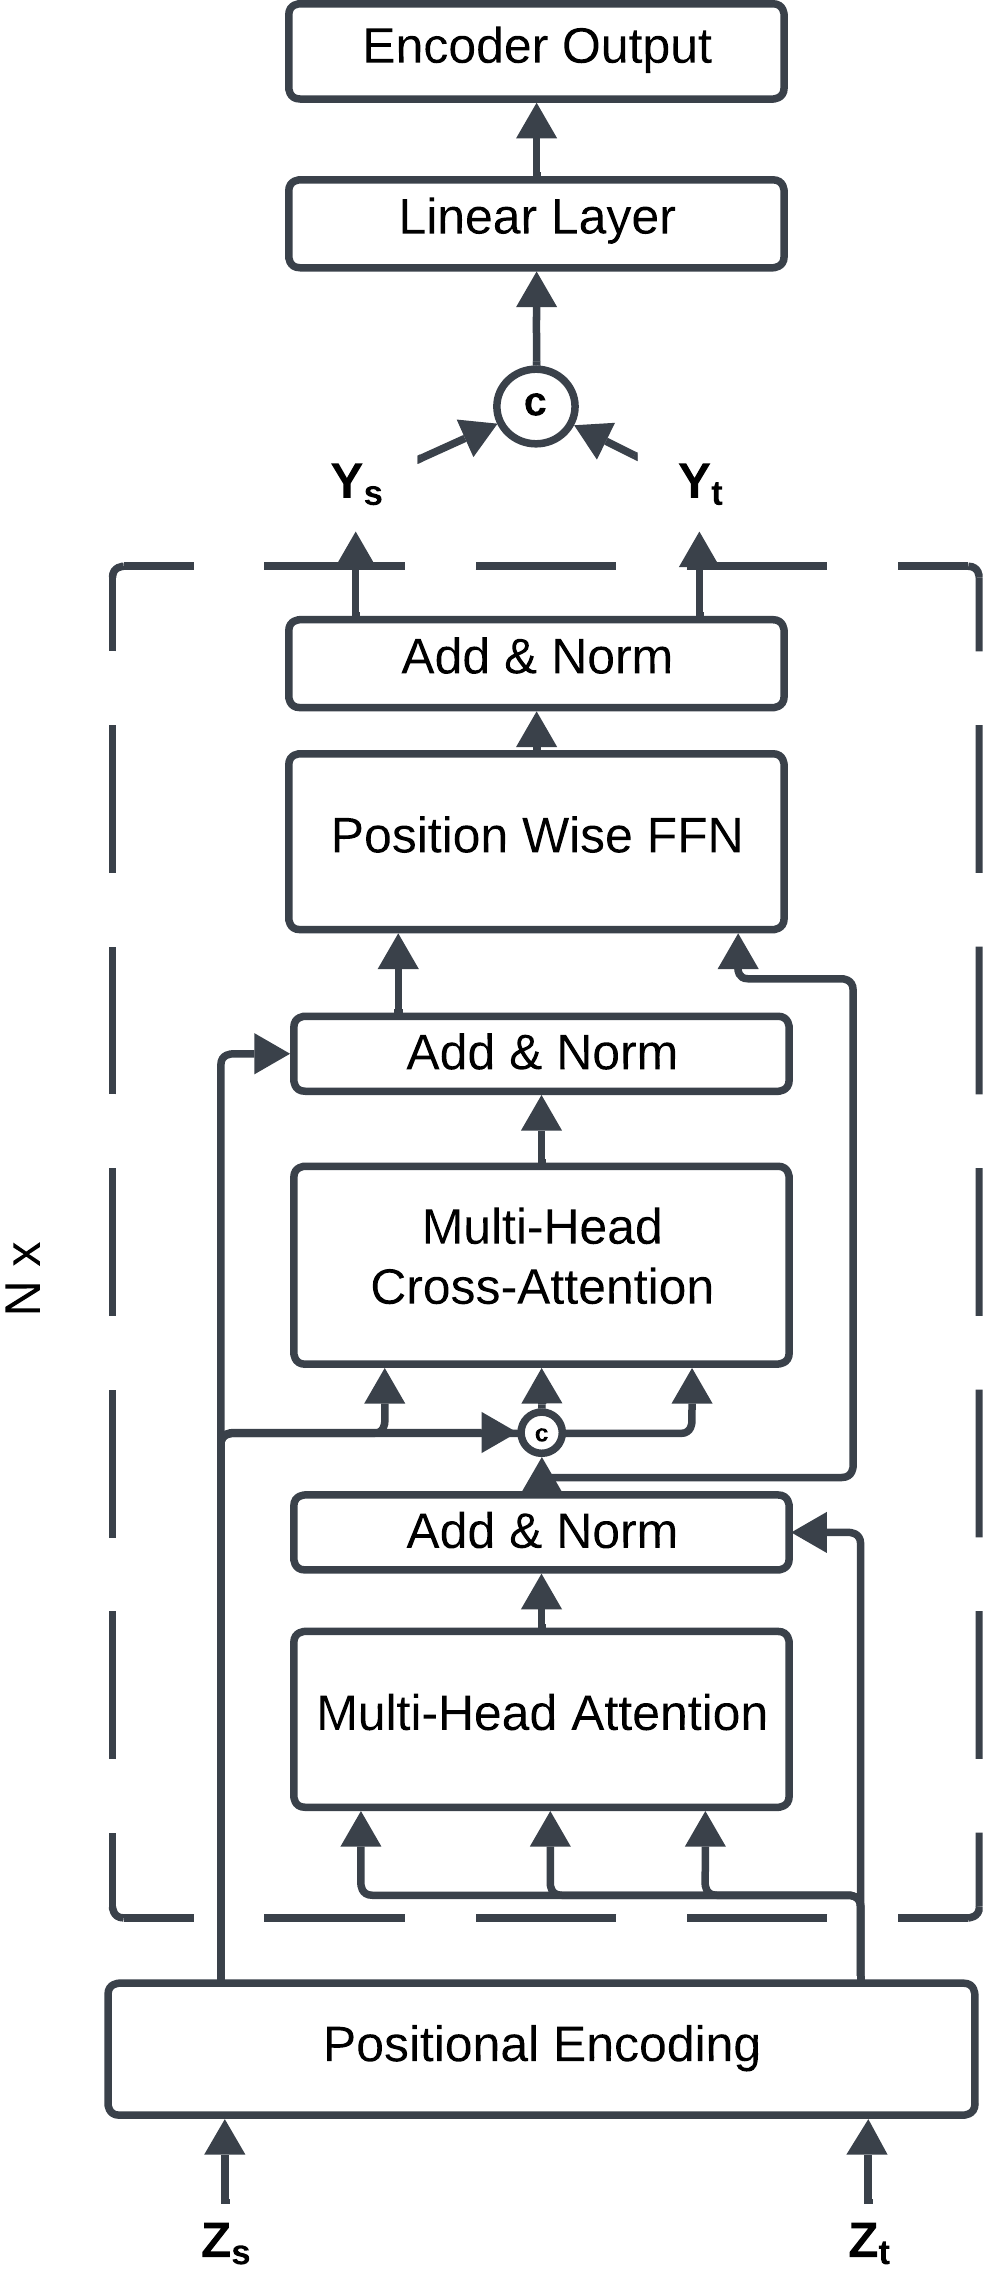
\includegraphics[width=0.4\linewidth]{gambar/Transformer Encoder.png}
    \caption{Encoder Cross Attention}
    \label{fig:crosss-attention}
\end{figure}

    \section{\textit{Self-Attention} dan \textit{Multi-Head Attention}}
     Proses dari \textit{Self-Attention} atau yang memiliki nama lain \textit{Scaled Dot-Product Attention} dapat dilihat pada Gambar \ref{fig:self_attention}.
\begin{figure}[H]
    \centering
    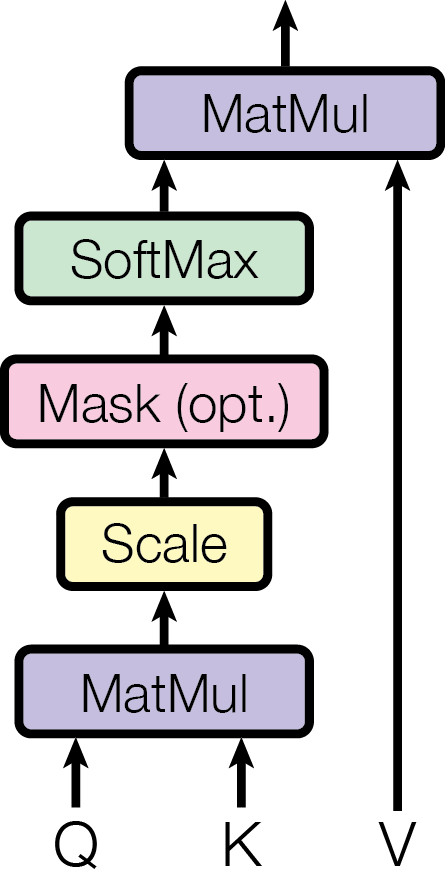
\includegraphics[width=0.25\linewidth]{gambar/ModalNet-19.png}
    \caption{\textit{Self-Attention} atau \textit{Scaled Dot-Product Attention}}
    \label{fig:self_attention}
\end{figure}

Proses dari \textit{Multi-Head Attention} dapat dilihat pada Gambar \ref{fig:multi_head_attention}.
\begin{figure}[H]
    \centering
    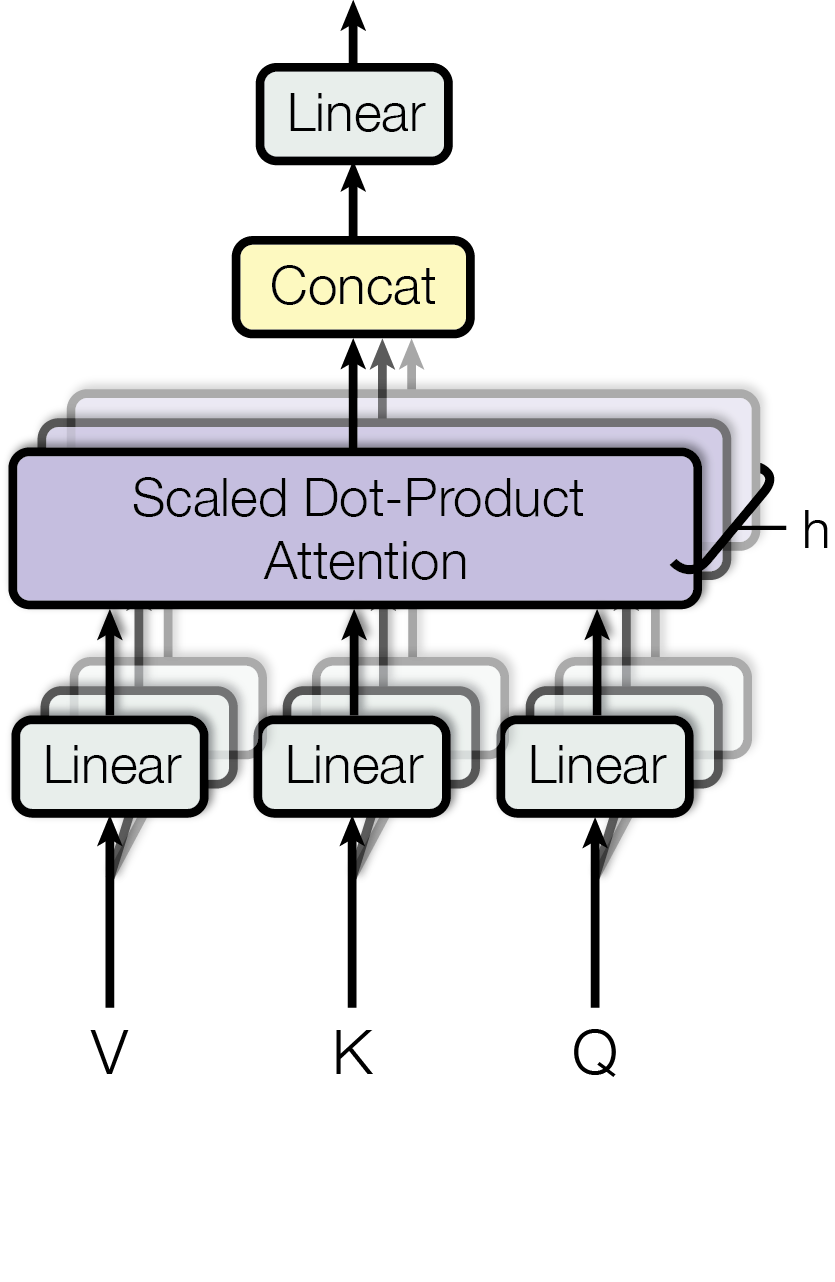
\includegraphics[width=0.38\linewidth]{gambar/ModalNet-20.png}
    \caption{\textit{Multi-Head Attention}}
    \label{fig:multi_head_attention}
\end{figure}

Inisiasi nilai variabel diperlukan untuk penentuan nilai awal pada pelatihan. Nilai yang digunakan adalah nilai yang sama dengan paper \textit{"Attention Is All You Need"} dengan beberapa penyesuaian \cite{vaswani2023attentionneed}. Nilai variabel inisiasi dapat dilihat pada tabel \ref{tab:transformer_encoder_vars}.
\begin{table}[H]
    \centering
    \caption{Tabel Variabel untuk Encoder Transformator}
    \begin{tabular}{l c}
        \hline
        \textbf{Nama Variabel} & \textbf{Nilai Variabel} \\ \hline
        EMBED\_DIM & 64 \\ \hline
        SEQ\_LENGTH & 512 \\ \hline
        NUM\_FEATURE & 8 \\ \hline
        D\_MODELS & 8 \\ \hline
        NUM\_HEADS & 8 \\ \hline
        DROPOUT\_RATE & 0.2 \\ \hline
        EPOCHS & 30 \\ \hline
    \end{tabular}
    \label{tab:transformer_encoder_vars}
\end{table}

Matriks fitur riwayat pasien $Z_t$ berukuran $8\times1$ dimasukkan ke dalam layer linear agar memiliki dimensi yang sama dengan matriks hasil ekstraksi fitur MFCC sehingga memiliki ukuran $8\times64$. Matriks fitur suara $Z_s$ hasil ekstraksi fitur MFCC berukuran $512\times64$ dan matriks fitur riwayat pasien berukuran $8\times64$ ditambahkan dengan token [cls] menjadi masing-masing berukuran $513\times64$ dan $9\times64$.

Matriks fitur riwayat pasien lalu masuk ke dalam mekanisme \textit{Multi-Head Attention} dan \textit{Layer Norm} dengan hasil matriks berukuran $9\times64$. Matriks ini selanjutnya di \textit{concat} dengan matriks fitur suara yang telah ditambah token [cls] berukuran $513\times64$ sehingga menghasilkan matriks berukuran $521\times64$.

Matriks fitur suara yang telah di \textit{concat} dengan matriks fitur riwayat pasien yang telah melalui mekanisme \textit{Multi-Head Attention} lalu masuk ke dalam mekanisme \textit{Multi-Head Cross Attention}. Operasi yang digunakan pada \textit{Multi-Head Cross Attention} sama dengan \textit{Multi-Head Attention}, perbedaannya terletak pada input berupa gabungan antara fitur suara dan fitur riwayat pasien. Setelah melewati \textit{Layer Norm} ukuran matriks hasil \textit{Multi-Head Cross Attention} menjadi $513\times64$.

\section{\textit{Feed-Forward Network}}
Matriks hasil \textit{Multi-Head Attention} dan \textit{Multi-Head Cross Attention} masing-masing masuk ke dalam mekanisme \textit{Feed-Forward Network}. mekanisme \textit{Feed-Forward Network} terdiri dari tiga operasi utama yaitu \textit{Linear Transformation}, \textit{Activation Function} dan \textit{Layer Normalization}. Transformasi Linear diimplementasikan sebagai \textit{fully connented layer}, atau juga dikenal sebagai \textit{dense layer}, yang menghubungkan setiap neuron masukan ke setiap neuron keluaran. Langkah berikutnya dalam operasi \textit{Feed-Forward Network} adalah menerapkan fungsi aktivasi. Fungsi ini merupakan fungsi non-linier yang memungkinkannya mempelajari pola yang lebih kompleks. Fungsi aktivasi yang digunakan pada model ini adalah GELU (\textit{Gaussian Error  Linear Unit}) yang memiliki kecepatan dan konvergensi yang lebih baik karena telah menggabungkan properti dari dropout, zoneout, dan ReLUs \cite{hendrycks2023gaussianerrorlinearunits}. Persamaan fungsi aktivasi GELU dapat dilihat pada persamaan \ref{eq:gelu}.

\begin{equation}
    \text{GELU}(x) = x P(X \leq x) = x \Phi(x) = x \cdot \frac{1}{2} \left[ 1 + \operatorname{erf}(x / \sqrt{2}) \right]
    \label{eq:gelu}
\end{equation}

Fungsi aktivasi GELU dapat diaproksimasi dengan persamaan \ref{eq:approx_gelu_1}
\begin{equation}
    0.5x(1 + \tanh[\sqrt{2/\pi}(x + 0.044715x^3)])
    \label{eq:approx_gelu_1}
\end{equation}
atau persamaan \ref{eq:approx_gelu_2}.
\begin{equation}
    x\sigma(1.702x)
    \label{eq:approx_gelu_2}
\end{equation}

Tahap terakhir pada \textit{Feed-Forward Network} adalah \textit{Layer Normalization}. \textit{Layer Normalization} adalah teknik yang menormalkan masukan di seluruh dimensi fitur (bukan dimensi batch), menstabilkan jaringan dan mempercepat pelatihan. Output dari \textit{Feed-Forward Network} berupa kedua matriks dengan ukuran $513\times64$ dan $9\times64$.

\section{Output Encoder $Y_s$ dan $Y_t$}
Proses dari keseluruhan di atas merupakan proses dalam satu blok encoder, proses ini diulang sebanyak N\_BLOCK. Didapatkan vektor $Y_s$ dan $Y_t$ dengan ukuran $1\times64$ yang kemudian di \textit{concat} secara horizontal/kolom sehingga didapatkan vektor berukuran $1\times128$. Vektor ini kemudian masuk ke dalam fungsi aktivasi GELU dan layer Linear sehingga didapatkan vektor berukuran $1\times64$. Fungsi aktivasi Softmax digunakan untuk mengakomodir klasifikasi multi-kelas dengan menghasilkan probabilitas setiap kelas dengan jumlah semua probabilitas berjumlah tepat 1. Fungsi aktivasi Softmax dapat dilihat pada persamaan \ref{eq:softmax}.
% Requires: \usepackage{amsmath}
\begin{equation}
    \sigma(\mathbf{z})_i = \frac{e^{z_i}}{\sum_{j=1}^{K} e^{z_j}}, \quad \text{for } i = 1, \ldots, K
    \label{eq:softmax}
\end{equation}
Keterangan:
\begin{itemize}
    \item $\sigma$ adalah softmax
    \item $\mathbf{z}$ adalah input vektor
    \item $K$ adalah jumlah kelas
    \item $e^{z_i}$ fungsi eksponensial untuk vektor input
    \item $e^{z_j}$ fungsi eksponensial untuk vektor output
\end{itemize}
Fungsi \ref{eq:softmax} menghasilkan vektor $1\times3$ yang berisi nilai probabilitas dari ketiga kelas. Nilai probabilitas terbesar menunjukkan prediksi kelas dari data.

\phantomsection%<---
\chapter{\textit{Optimizer Adam}} \label{lam:lampiran_a}
    \section{Optimizer Adam pada Transformers}
    Adam menggabungkan kelebihan dari dua algoritma optimisasi yaitu momentum dan RMSProp dengan mengestimasi rata-rata dan varians dari gradien. Dalam model Transformers, parameter $\theta$ mencakup bobot dan bias untuk:
\begin{itemize}
    \item Lapisan \textit{self-attention} dan \textit{multi-head attention} (seperti bobot proyeksi query, key dan value).
    \item \textit{Feed-Forward Network}.
    \item Parameter \textit{Layer Normalization}.
\end{itemize}
Setiap parameter diperbarui menggunakan persamaan di bawah.

\subsection{Persamaan Oprimizer Adam}

1. Menghitung gradien dari loss \( L \) dengan parameter \( \theta \) dengan persamaan \ref{eq:gradien_loss}:
\begin{equation}
    g_t = \nabla_{\theta} L(\theta_t)
    \label{eq:gradien_loss}
\end{equation}

2. Perbarui estimasi momentum bias dengan persamaan \ref{eq:mean_gradien}dan \ref{eq:varian_gradien}:
\begin{equation}
    m_t = \beta_1 m_{t-1} + (1 - \beta_1) g_t
    \label{eq:mean_gradien}
\end{equation}
\begin{equation}
    v_t = \beta_2 v_{t-1} + (1 - \beta_2) g_t^2
    \label{eq:varian_gradien}
\end{equation}

3. Terapkan koreksi bias pada momentum dengan persamaan \ref{eq:bias_correction}:
\begin{equation}
    \hat{m}_t = \frac{m_t}{1 - \beta_1^t}, \quad \hat{v}_t = \frac{v_t}{1 - \beta_2^t}
    \label{eq:bias_correction}
\end{equation}
4. Perbarui parameter dengan persamaan \ref{eq:update_param}:
\begin{equation}
    \theta_{t+1} = \theta_t - \eta \frac{\hat{m}_t}{\sqrt{\hat{v}_t} + \epsilon}
    \label{eq:update_param}
\end{equation}
Keterangan:
\begin{itemize}
    \item $g_t$ adalah fungsi gradien
    \item $L(\theta_t)$ adalah fungsi Loss
    \item $m_t$ adalah momentum
    \item $v_t$ adalah velocity
    \item $\eta$ merupakan \textit{learning rate}.
    \item $\beta_1$ dan $\beta_2$ adalah \textit{hyperparameter} yang mengendalikan tingkat peluruhan estimasi momen.
    \item $\epsilon$ adalah konstanta kecil untuk mencegah pembagian dengan nol.
\end{itemize}


\subsection{Contoh Perhitungan}
Asumsikan :

\begin{itemize}
  \item Learning rate $\eta = 0.001$,
  \item $\beta_1 = 0.9$, $\beta_2 = 0.999$,
  \item $\epsilon = 10^{-8}$,
  \item Gradien pada \textit{timestep} $t$: $g_t = 0.02$,
  \item Estimasi momentum sebelumnya: $m_{t-1} = 0.01$, $v_{t-1} = 0.0001$,
  \item $t = 10$.
\end{itemize}


Langkah-langkah perhitungan:

1. Hitung estimasi momen bias:
\[
m_t = \beta_1 m_{t-1} + (1 - \beta_1) g_t = 0.9 \cdot 0.01 + (1 - 0.9) \cdot 0.02 = 0.011
\]
\[
v_t = \beta_2 v_{t-1} + (1 - \beta_2) g_t^2 = 0.999 \cdot 0.0001 + (1 - 0.999) \cdot (0.02)^2 = 0.0001004
\]

2. Terapkan koreksi bias:
\[
\hat{m}_t = \frac{m_t}{1 - \beta_1^t} = \frac{0.011}{1 - 0.9^{10}} \approx 0.0111
\]
\[
\hat{v}_t = \frac{v_t}{1 - \beta_2^t} = \frac{0.0001004}{1 - 0.999^{10}} \approx 0.000102
\]

3. Hitung pembaruan parameter:
\[
\Delta \theta = \eta \frac{\hat{m}_t}{\sqrt{\hat{v}_t} + \epsilon}
\]
Subsitusikan nilai:
\[
\Delta \theta = 0.001 \cdot \frac{0.0111}{\sqrt{0.000102} + 10^{-8}} \approx 0.00109
\]

4. Perbarui parameter:
\[
\theta_{t+1} = \theta_t - \Delta \theta
\]

\phantomsection%<---
\chapter{Variasi Model dan \textit{Hyperparameter Tuning}} \label{lampiran B}
 \begin{table}[ht]
    \centering
    \caption{Variasi Model dan Hyperparameter Transformer}
    \begin{tabular}{@{}lcc@{}}
        \toprule
        \textbf{Hyperparameter} & \textbf{Small Model} & \textbf{Big Model} \\ \midrule
        Jumlah Layer/Blok Encoder ($N\_BLOCK$)      & 6                   & 12                 \\
        Dimensi Embedding ($d_\text{model}$) & 64                 & 128               \\
        Dimensi Feedforward ($d_\text{ff}$) & 256                & 512               \\
        Jumlah Head Attention  & 8                   & 16                 \\
        Dropout                & 0.2                 & 0.3                \\
        Batch Size             & 32                  & 64                \\
        Learning Rate          & 1e-4                & 5e-5               \\ \bottomrule
    \end{tabular}
    \label{tab:transformer-variations}
\end{table}
\end{appendix}

\end{document}